%%%%%%%%%%%%%%%%%%%%%%%%% 
% Dokumentinformationen %
%%%%%%%%%%%%%%%%%%%%%%%%%
\newcommand{\titleinfo}{Signale und Systeme 1 - Zusammenfassung}
\newcommand{\authorinfo}{Braun \& Co, J.Rast, C.Gwerder, S.K\"orner}
\newcommand{\versioninfo}{$Revision: 1 $ - powered by \LaTeX} 

%%%%%%%%%%%%%%%%%%%%%%%%%%%%%%%%%%%%%%%%%%%%%
% Standard projektübergreifender Header für
% - Makros 
% - Farben
% - Mathematische Operatoren
%
% DORT NUR ERGÄNZEN, NICHTS LÖSCHEN
%%%%%%%%%%%%%%%%%%%%%%%%%%%%%%%%%%%%%%%%%%%%%
% Genereller Header
\documentclass[10pt,twoside,a4paper,fleqn]{article}
% Dateiencoding
\usepackage[utf8]{inputenc}
% Seitenränder
\usepackage[left=1cm,right=1cm,top=1cm,bottom=1cm,includeheadfoot]{geometry}
% Sprachpaket
\usepackage[ngerman]{babel,varioref}

% Pakete
\usepackage{amssymb,amsmath,fancybox,graphicx,lastpage,wrapfig,fancyhdr,hyperref,verbatim,floatflt,multicol,multirow,rotating,pdflscape,array,longtable,listings}

% Zum Bilder einfach in Tabellen einfügen (valign=t)
\usepackage[export]{adjustbox}

%%%%%%%%%%%%%%%%%%%%
% Generelle Makros %
%%%%%%%%%%%%%%%%%%%%
\newcommand{\skript}[1]{$_{\textcolor{red}{\mbox{\small{Skript S.#1}}}}$}
\newcommand{\verweis}[2]{\small{(siehe auch \ref{#1}, #2 (S. \pageref{#1}))}}
\newcommand{\verweiskurz}[1]{(\small{siehe \ref{#1}\normalsize)}}
\newcommand{\subsubadd}[1]{\textcolor{black}{\mbox{#1}}}
\newcommand{\formelbuch}[1]{$_{\textcolor{red}{\mbox{\small{S#1}}}}$}

\newcommand{\kuchling}[1]{$_{\textcolor{red}{\mbox{\small{Kuchling #1}}}}$}
\newcommand{\stoecker}[1]{$_{\textcolor{orange}{\mbox{\small{Stöcker #1}}}}$}
\newcommand{\sachs}[1]{$_{\textcolor{blue}{\mbox{\small{Sachs S. #1}}}}$}
\newcommand{\hartl}[1]{$_{\textcolor{green}{\mbox{\small{Hartl S. #1}}}}$}

\newcommand{\schaum}[1]{\tiny Schaum S. #1}

\newcommand{\skriptsection}[2]{\section{#1 {\tiny Skript S. #2}}}
\newcommand{\skriptsubsection}[2]{\subsection{#1 {\tiny Skript S. #2}}}
\newcommand{\skriptsubsubsection}[2]{\subsubsection{#1 {\tiny Skript S. #2}}}

\newcommand{\matlab}[1]{\footnotesize{(Matlab: \texttt{#1})}\normalsize{}}

%%%%%%%%%%
% Farben %
%%%%%%%%%%
\usepackage{xcolor}

%%%%%%%%%%%%%%%%%%%%%%%%%%%%
% Mathematische Operatoren %
%%%%%%%%%%%%%%%%%%%%%%%%%%%%
\DeclareMathOperator{\sinc}{sinc}
\DeclareMathOperator{\sgn}{sgn}
\DeclareMathOperator{\Real}{Re}
\DeclareMathOperator{\Imag}{Im}
%\DeclareMathOperator{\e}{e}
\DeclareMathOperator{\cov}{cov}
\DeclareMathOperator{\PolyGrad}{PolyGrad}

%Makro für 'd' von Integral- und Differentialgleichungen 
\newcommand*{\diff}{\mathop{}\!\mathrm{d}}


%%%%%%%%%%%%%%%%%%%%%%%%%%%
% Fouriertransformationen %
%%%%%%%%%%%%%%%%%%%%%%%%%%%
\usepackage{trfsigns, trsym}
%\unitlength1cm
% Zeitbereich -- Frequenzbereich
%\newcommand{\laplace}
%{
%\begin{picture}(1,0.5)
%\put(0.2,0.1){\circle{0.14}}\put(0.27,0.1){\line(1,0){0.5}}\put(0.77,0.1){\circle*{0.14}}
%\end{picture}
%}
% Frequenzbereich -- Zeitbereich
%\newcommand{\Laplace}
%{
%\begin{picture}(1,0.5)
%\put(0.2,0.1){\circle*{0.14}}\put(0.27,0.1){\line(1,0){0.45}}\put(0.77,0.1){\circle{0.14}}
%\end{picture}
%}


% Fouriertransformationen
\unitlength1cm
\newcommand{\FT}
{
\begin{picture}(1,0.5)
\put(0.2,0.1){\circle{0.14}}\put(0.27,0.1){\line(1,0){0.5}}\put(0.77,0.1){\circle*{0.14}}
\end{picture}
}


\newcommand{\IFT}
{
\begin{picture}(1,0.5)
\put(0.2,0.1){\circle*{0.14}}\put(0.27,0.1){\line(1,0){0.45}}\put(0.77,0.1){\circle{0.14}}
\end{picture}
}




%%%%%%%%%%%%%%%%%%%%%%%%%%%%
% Allgemeine Einstellungen %
%%%%%%%%%%%%%%%%%%%%%%%%%%%%
%PDF Info
\hypersetup{pdfauthor={\authorinfo},pdftitle={\titleinfo},colorlinks=false}
\author{\authorinfo}
\title{\titleinfo}

%%%%%%%%%%%%%%%%%%%%%%%
% Kopf- und Fusszeile %
%%%%%%%%%%%%%%%%%%%%%%%
\pagestyle{fancy}
\fancyhf{}
%Linien oben und unten
\renewcommand{\headrulewidth}{0.5pt} 
\renewcommand{\footrulewidth}{0.5pt}

\fancyhead[L]{\titleinfo{ }\tiny{(\versioninfo)}}
%Kopfzeile rechts bzw. aussen
\fancyhead[R]{Seite \thepage { }von \pageref{LastPage}}
%Fusszeile links bzw. innen
\fancyfoot[L]{\footnotesize{\authorinfo}}
%Fusszeile rechts bzw. ausen
\fancyfoot[R]{\footnotesize{\today}}
% Lizenz CC-BY-NC-SA
% Headerfile für die Einbindung einer Lizenzgrafik in den Footer
% Verwendung: \lizenz{cc-by-nc-sa}{small}
\newcommand{\lizenz}[2]
{
\fancyfoot[C]{
  \includegraphics[width=1.6cm]{./header/lizenzen/#1/#2.png}
}
}
\lizenz{cc-by-nc-sa}{small}
% Einrücken verhindern versuchen
\setlength{\parindent}{0pt}

% Zeilenhöhe Tabellen:
\newcommand{\arraystretchOriginal}{1.5}
\renewcommand{\arraystretch}{\arraystretchOriginal}


\usepackage{pdfpages}

% Möglichst keine Ergänzungen hier, sondern in header.tex
\begin{document}
\title{\Huge{SigSys 1}}
\maketitle
\tableofcontents
\newpage

\section{Signalbeschreibung \skript{1}}
	\renewcommand{\arraystretchOriginal}{1}
	
	\subsection{Signalklassen \skript{2}}
	
		\begin{tabular}{|l|c|l|}
		\hline 
		periodisch & $\Longleftrightarrow$ & nicht-periodisch \\ 
		\hline 
		kontinuierlich & $\Longleftrightarrow$ & zeitdiskret \\ 
		\hline 
		analog & $\Longleftrightarrow$ & digital \\ 
		\hline 
		reell & $\Longleftrightarrow$ & komplex \\ 
		\hline 
		eindimensional & $\Longleftrightarrow$ & mehrdimensional \\ 
		\hline 
		deterministisch & $\Longleftrightarrow$ & stochastisch \\ 
		\hline 
		\end{tabular}


		\subsubsection{Energie- und Leistungssignale \skript{3}}
		
			\begin{tabularx}{\textwidth}{|p{3.1cm}|c|c|c|}
			\hline
				{}
			&	\multirow{2}{*}{Klasse 1: Energiesignale}
			&	\multicolumn{2}{c|}{Klasse 2: Leistungssignale}
			\\ 
				{}
			&	
			&	Klasse 2a: periodisch
			&	Klasse 2b: aperiodisch
			\\ \hline 
				{}
			&	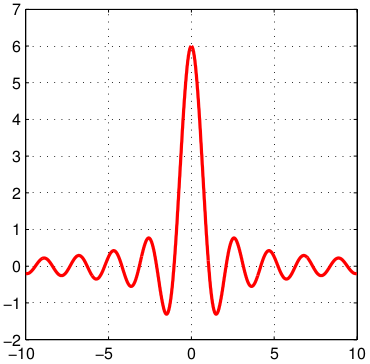
\includegraphics[width=3.3cm]{./bilder/sinc.png}
			& 	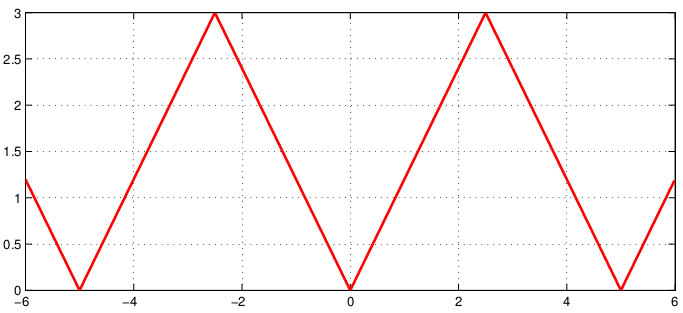
\includegraphics[width=3.5cm]{./bilder/dreieck.png}
			& 	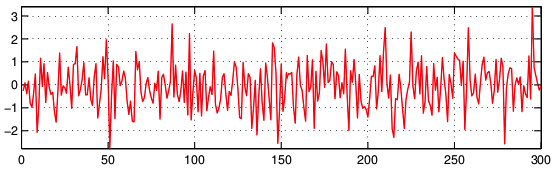
\includegraphics[width=5.29cm]{./bilder/rauschen.png}
			\\ \hline 
				Energie-/Leistungs-dichtesprektrum
			& 	$ E(j \omega) = |F(j \omega)|^2 $
			& 	\multicolumn{2}{c|}{$ \Phi(j\omega) = \lim\limits_{T \to \infty} \dfrac{|F(j\omega)|^2}{T} $}
			\\ \hline 
				Normierte
			& 	$ P_n = 0$
			& 	\formel{$P_n = X^2$} (quadr. Mittelwert)
			& 	$ P_n = \lim\limits_{T \rightarrow \infty} \frac{1}{T} 
									\int\limits_{-T/2}\limits^{T/2} |f(t)|^2 dt $
			\\
				Signalleistung
			&
			& 	(Formeln rechts gelten auch)
			& 	$ P_n = \dfrac{1}{2\pi} \cdot \int\limits_{-\infty}^{\infty} \Phi(j\omega) d\omega $
			\\ \hline
				Normierte
			& 	$ W_n = \lim\limits_{T \rightarrow \infty} \int\limits_{-T/2}\limits^{T/2} |f(t)|^2 dt $
			&	\multicolumn{2}{c|}{$ W_n = \infty $}
			\\
				Signalenergie
			& 	$ W_n = \frac{1}{2 \pi} \int\limits_{-\infty}\limits^{\infty}
									W(j \omega) d\omega $
			&	\multicolumn{2}{c|}{}
			\\ \hline
			\end{tabularx}
		
		
	\subsection{Mittelwerte \skript{5}}
		
		\begin{tabularx}{\textwidth}{p{4.7cm}p{8.1cm}X}
			Arithmetischer Mittelwert, Gleichwert, Linearer MW
		&	$X_0 = \overline{X} = X_m = \frac {1} {T} \int\limits_{-T/2}^{T/2} x(t)dt$
		&	Ist die Fläche unter der Zeitfunktion über eine Periode, nur Klasse 2a
		\\
		    {}
		&   $X_0 = \lim\limits_{T\rightarrow \infty}{\frac {1} {T} \int\limits_{-T/2}^{T/2} x(t)dt}$
		&   nur Klasse 2b
		\\
			Quadratischer MW, Leistung
		&	$X^2 = \frac {1} {T} \int\limits_{-T/2}^{T/2} x^2(t)dt$
		& 	nur Klasse 2a
		\\
			Mittelwert n. Ordnung
		&	$X^n = \frac {1} {T} \int\limits_{-T/2}^{T/2} x^n(t)dt$
		& 	nur Klasse 2a
		\\
			Effektivwert
		&	$X = X_{\text{eff}}= \sqrt{X^2} = \sqrt{\frac{1}{T} \int\limits_{-T/2}^{T/2}{x^2(t)dt}}$
		&	nur Klasse 2a
		\\
			Gleichrichtwert
		&	$X_{|m|} = \bar{|X|} = \frac{1}{T} \int\limits_{-T/2}^{T/2}{|x(t)| dt}$
		&	Arithm. Mittelwert der Zweiweggleichrichterschaltung
	    \\
			Varianz, Standardabweichung
		&	$\text{Var}(x)=\sigma^2= \frac {1} {T} \int\limits_{-T/2}^{T/2}(x(t)-X_0)^2dt = X^2-X_0^2$
		&	Mittlerer Fehler im Quadrat
		\\
		\end{tabularx} \\
	
		\textbf{Hinweis:} \\
		\begin{tabularx}{\textwidth}{llX}
			Für \textbf{reelle Signale} gilt: &
			$ X^2 = |X|^2 = Var(|x|) + |X_0|^2 $ &
			Dies kann die Berechnung des quadratischen Mittelwertes eines zum linearen Mittelwert symmetrischen Signales erleichtern.
		\end{tabularx}
		
		
	\subsection{Autokorrelationsfunktion (AKF) \skript{8}} 
	Die Autokorrelation ist ein Mass für die innere Kohärenz (Ähnlichkeit) eines Signals (Wie weit wird die Zukunft von der Vergangenheit geprägt?).
	
		\bgroup
		\setlength{\tabcolsep}{1mm}
		\begin{tabularx}{\textwidth}{|cX|cX|cX|}
		\hline 
			\multicolumn{2}{|c|}{\textbf{Energiesignale} (Klasse 1)} &
			\multicolumn{2}{|c|}{\textbf{periodische Leistungssignale} (2a)} & 
			\multicolumn{2}{|c|}{\textbf{stochastische Leistungssignale} (2b)}
		\\ \hline 
			$ \varphi_{xx}(\tau) $ &
			$ 		= \lim\limits_{T\to\infty}\int\limits_{-T/2}^{T/2} x(t)x(t-\tau)dt $ \linebreak
				$ 	= \lim\limits_{T\to\infty}\int\limits_{-T/2}^{T/2} x(t+\tau)x(t)dt $ \linebreak
				$	= \varphi_{xx}(-\tau)$ &
			$ \varphi_{xx}(\tau) $ &
			$ 		= \frac {1} {T} \int\limits_{-T/2}^{T/2} x(t)x(t-\tau)dt $ \linebreak
				$	= \frac {1} {T} \int\limits_{-T/2}^{T/2} x(t+\tau)x(t)dt $ \linebreak
				$	= \varphi_{xx}(-\tau) $ &
			$ \varphi_{xx}(\tau) $ &
			$		= \lim\limits_{T\rightarrow\infty} \frac {1} {T} \int\limits_{-T/2}^{T/2} x(t)x(t-\tau)dt $ \linebreak
				$	= \lim\limits_{T\rightarrow\infty}\frac {1} {T} \int\limits_{-T/2}^{T/2} x(t+\tau)x(t)dt $ \linebreak
				$ = \varphi_{xx}(-\tau) $
		\\ \hline
		\end{tabularx} 
		\egroup
		
		\begin{tabularx}{\textwidth}{lX}
		\parbox{6cm}{
			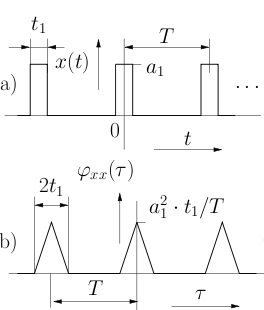
\includegraphics[width=4cm]{./bilder/akf1.png}\\
			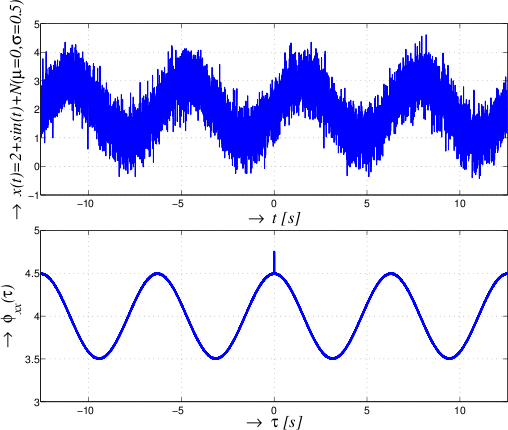
\includegraphics[width=4cm]{./bilder/akf2.png}
		} 
		&
		\parbox{12cm}{
			\textbf{Eigenschaften}
			\begin{itemize}
     			\item $\varphi_{xx}(0) = X^2 = (X_0)^2+\sigma^2$ (Hat immer Diracstoss bei $\tau = 0$)
     			\item $\varphi_{xx}(\tau)=\varphi_{xx}(\tau\pm mT)$, d.h. die AKF
     				ist periodisch mit der gleichen Periode $T$ wie das Signal $x(t)$.
				\item $\varphi_{xx}(\tau)=\varphi_{xx}(-\tau)$: d.h. die AKF ist eine {\bf gerade Funktion}
				\item $\varphi_{xx}(0)\geq|\varphi_{xx}(\tau)|\quad$
				\item $\varphi_{xx}(\tau)\geq (X_0)^2-\sigma^2\quad$
   			\end{itemize}
   			
   			\textbf{Für Leistungssignale gilt:} \ \ \textit{$\Phi(j\omega)$: Leistungsdichtespektrum} \\
   			\fbox{$ \dfrac{1}{2\pi} \cdot \int\limits_{-\infty}^{\infty} \Phi(j\omega) \cdot \e^{j\omega t} d\omega 
						= \colorbox{yellow}{$\varphi_{xx}(t) \ \laplace \ \Phi(j\omega)$} =
						\int\limits_{-\infty}^{\infty} \varphi_{xx}(t) \cdot \e^{-j\omega t} dt $}\\
						
			\textbf{Für Energiesignale gilt:} \ \ \textit{$E(j\omega)$: Energiedichtespektrum} \\
   			\fbox{$ \dfrac{1}{2\pi} \cdot \int\limits_{-\infty}^{\infty} E(j\omega) \cdot \e^{j\omega t} d\omega 
						= \colorbox{yellow}{$\varphi_{xx}(t) \ \laplace \ E(j\omega)$} =
						\int\limits_{-\infty}^{\infty} \varphi_{xx}(t) \cdot \e^{-j\omega t} dt $}\\
   
   			\textbf{Beispiele}
   			\begin{itemize}
     			\item $x(t) = a_k \cos(\omega t + \varphi) \Rightarrow \varphi_{xx}(t) = \frac{a_k^2}{2} \cos(\omega t)$
     			\item $x(t) = b_k \sin(\omega t + \varphi) \Rightarrow \varphi_{xx}(t) = \frac{b_k^2}{2} \cos(\omega t)$
   			\end{itemize}
   		} \\
		\end{tabularx}
				
	\subsection{Kreuzkorrelationsfunktion (KKF) \skript{11}} 
		Die Kreuzkorrelationsfunktion von periodischen Leistungssignalen (Klasse 2a) ist ein Mass für die Ähnlichkeit von zwei verschiedenen Signalen . \textit{''Wie ähnlich sind sich zwei Signale?'' \ \matlab{xcorr}}
		\\	
		\bgroup
		\setlength{\tabcolsep}{1mm}
		\begin{tabularx}{\textwidth}{|cX|cX|cX|}
		\hline 
			\multicolumn{2}{|c|}{\textbf{Energiesignale} (Klasse 1)} &
			\multicolumn{2}{|c|}{\textbf{periodische Leistungssignale} (2a)} & 
			\multicolumn{2}{|c|}{\textbf{stochastische Leistungssignale} (2b)}
		\\ \hline 
			$ \varphi_{xy}(\tau) $ &
			$ 		= \lim\limits_{T\to\infty}\int\limits_{-T/2}^{T/2} x(t)y(t-\tau)dt $ \linebreak
				$ 	= \lim\limits_{T\to\infty}\int\limits_{-T/2}^{T/2} x(t+\tau)y(t)dt $ &
			$ \varphi_{xy}(\tau) $ &
			$ 		= \frac {1} {T} \int\limits_{-T/2}^{T/2} x(t)y(t-\tau)dt $ \linebreak
				$	= \frac {1} {T} \int\limits_{-T/2}^{T/2} x(t+\tau)y(t)dt $ &
			$ \varphi_{xy}(\tau) $ &
			$		= \lim\limits_{T\rightarrow\infty} \frac {1} {T} \int\limits_{-T/2}^{T/2} x(t)y(t-\tau)dt $ \linebreak
				$	= \lim\limits_{T\rightarrow\infty}\frac {1} {T} \int\limits_{-T/2}^{T/2} x(t+\tau)y(t)dt $
		\\ \hline
		\end{tabularx} 
		\egroup

		\begin{tabularx}{\textwidth}{llX}
		\parbox{2.9cm}{
			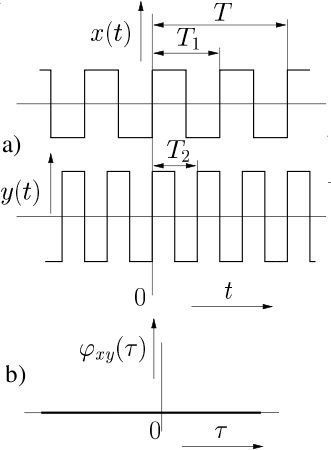
\includegraphics[width=2.9cm]{./bilder/kkf1.png}
		} 
		&
		\parbox{3.9cm}{
			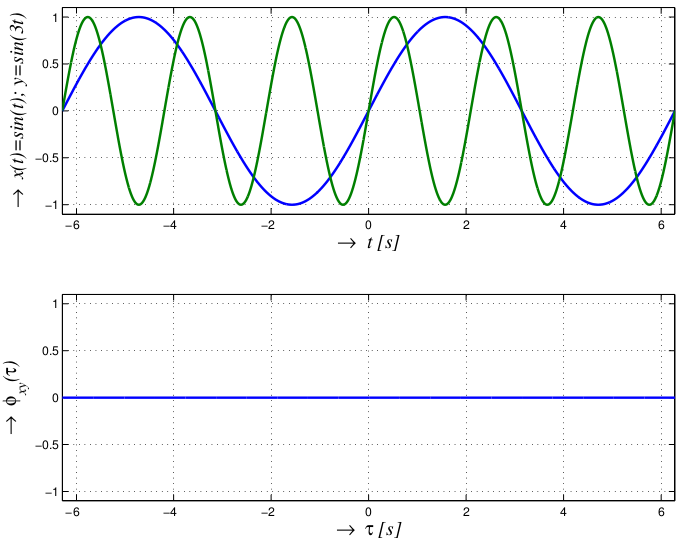
\includegraphics[width=3.9cm]{./bilder/kkf2.png}
		} 
		&
		\parbox{10cm}{
			\textbf{Eigenschaften}
			\begin{itemize}
     			\item Bei Signalen mit verschiedenen Frequenzen ist $\varphi_{xy}$ immer $0$!
     			\item Bei stochastischen Signalen ist $\varphi_{xy}$ immer $0$!
   			\end{itemize}
   			
   			\textbf{Für stochastische Leistungssignale (Klasse 2b) gilt:} \\
   			\fbox{$ \dfrac{1}{2\pi} \int\limits_{-\infty}^{\infty} \Phi_{xy}(j\omega) \e^{j\omega t} d\omega 
						= \colorbox{yellow}{$\varphi_{xy}(t) \ \laplace \ \Phi_{xy}(j\omega)$} =
						\int\limits_{-\infty}^{\infty} \varphi_{xy}(t) \e^{-j\omega t} dt $}\\
   		} \\
		\end{tabularx}
		
		
	\subsection{Rauschen \skript{25} \matlab{randn}}
	
		\begin{tabularx}{\textwidth}{lX}
			\parbox{8cm}{
				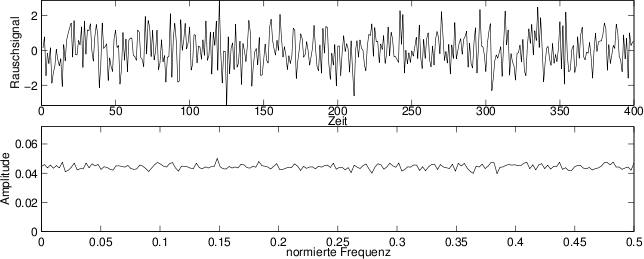
\includegraphics[width=8cm]{./bilder/rauschen2.png}
			} &
			\parbox{9.5cm}{
			Ist die Intensität der
			Rauschspannung "uber viele Frequenzdekaden
			gleich verteilt, so spricht man von weissem Rauschen.\\ \\
			\textbf{Ideale Blindwiderstände verursachen kein Rauschen!}
			\begin{itemize}
     			\item $\text{SNR} = \frac{P_s}{P_r} = \frac{\text{Signalleistung}}{\text{Rauschleistung}}$ (rauschfrei: $ \text{SNR} \rightarrow \infty$) 
     			\item Effektive Rauschspannung: \fbox{$U_r = \sqrt { 4 \cdot k \cdot T \cdot \Delta f \cdot R}$}
     			\item Effektive Rauschleistung: \fbox{$P_r = k \cdot T \cdot \Delta f$}
     			\item Bolzmann-Konstante: $k =1.380662 \cdot 10^{-23}\frac{J}{K}$
   			\end{itemize}
			}
		\end{tabularx}\\
		
	\subsection{Signal-Rausch-Verhältnis (SNR) \skript{27}}
	
		Zur Qualitätsbeurteilung von Signalen wird das Verhältnis zwischen der Leistung des Nutzsignales $P_s$ und der 
		des Rauschsignales $P_r$ gebildet. Dieses Verhältnis wird \textbf{Störabstand} oder \textbf{Rauschabstand} $a_r$ genannt.\\
	
		\begin{minipage}[]{10cm}
			\formel{$a_r = 10 \cdot log_{10} \left(\frac{P_s}{P_r}\right) = 20 \cdot log_{10} \left(\frac{U_s}{U_r}\right)$}
			$[a_r] = dB$\\
		\end{minipage}
		\begin{minipage}[]{10cm}		
			Mindestwert für eine rauschfreie Übertragung: \\
			Musik und Sprache $\rightarrow$ 30 dB \\
			Bilder $\rightarrow$ 40 dB
		\end{minipage}
	
	
	\subsection{Rauschzahl $F$ und Rauschmass $a_F$ \skript{27}}
	
		Jeder Vierpol verkleinert den Rauschabstand des Ausgangssignales gegenüber dem Rauschabstand des Eingangssignales.
		Die Verschlechterung des Rauschleistungsabstandes wird durch die Rauschzahl $F$ \textit{(noise figure)} angegeben.
		Es ist das Verhältnis des Rauschabstandes am Eingang zum Rauschabstand am Ausgang eines Vierpoles.\\
		
		\begin{tabular}{lll}
			\textbf{Rauschzahl:}
		&	\fbox{$F 	= \dfrac{\text{SNR}_{Eingang}}{\text{SNR}_{Ausgang}}
						= \dfrac{\frac{P_{sEingang}}{P_{rEingang}}}{\frac{P_{sAusgang}}{P_{rAusgang}}} 
						= \frac{P_{sEingang}}{P_{rEingang}} \cdot \frac{P_{rAusgang}}{P_{sAusgang}}$}
		&	Idealer Vierpol: $F = 1$
		\\
			\textbf{Rauschmass} (logarithmisch):
		&	\formel{$a_F = 10 \cdot log_{10} (F) = a_{rEingang} - a_{rAusgang}$}
		&	$[a_F] = dB$
		\end{tabular}\\
	
	\subsection{Amplitudenanalyse von Signalen \skript{29}}
	
		\begin{tabular}{ll}
			\parbox{7cm}{
				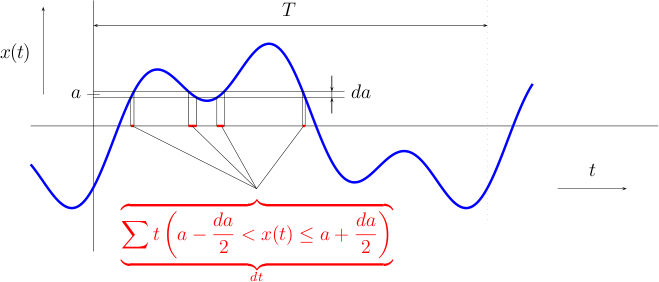
\includegraphics[width=7cm]{./bilder/amplitudenanalyse.png}
			}
		& 	\begin{minipage}[]{11cm}
			Die Amplitudendichte $p(a)$ ist ein Mass für u die relative Zeit ( Zeit / Gesamtzeit =	Wahrscheinlichkeit), während der sich das Signal in einem bestimmten Amplitudenintervall a +- da / 2 aufhält.
			''Zeit während sich Signal in bestimmtem Amplitudenintervall aufhält''\\
				\fbox{$p(a) 	= \lim\limits_{da \rightarrow 0}\frac{\underbrace{\sum t\left(
								a-\frac{da}{2}<x(t)\leq a+\frac{da}{2}\right)}_{dt}}{T\cdot da}
							= \frac{1}{T}\cdot\frac{dt}{da}$}\\
      		\end{minipage}
		\\
			\parbox{7cm}{
				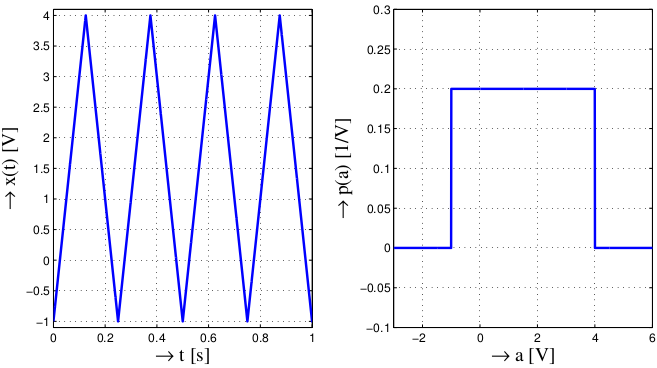
\includegraphics[width=7cm]{./bilder/amplitudenanalyse2.png}
			}
		& 	\begin{minipage}[]{11cm}
				\textbf{Eigenschaften}
				\begin{itemize}
					\item Es gibt keine negativen Werte! $p(a) \geq 0 \ \ \forall a$
     				\item \fbox{$\int\limits_{-\infty}^{\infty} p(a) da = 1$}
     				\item \fbox{$p(a_1 < a < a_2) = \int\limits_{a_1}^{a_2} p(a) da$}
   				\end{itemize}
				
      		\end{minipage}
		\end{tabular}\\ \\
	
		\begin{tabular}{ll}
        		\textbf{Linearer Mittelwert:} \fbox{$X_0  = \int\limits_{-\infty}^{\infty}a\cdot p(a)da$}
        	&	\textbf{Mittelwert $n$. Ordnung:} \fbox{$X^n = \int\limits_{-\infty}^{\infty}a^n\cdot p(a)da$}\\
        	&	\\
        		\textbf{Varianz:} \fbox{$Var(x)  = \int\limits_{-\infty}^{\infty}(a-X_0)^2 \cdot p(a)da$}
        	&
        \end{tabular}\\ \\
	
		\textbf{Beispiel:}\\
		\beispiel{
		\begin{tabularx}{\textwidth}{cX}
			\parbox{7cm}{
				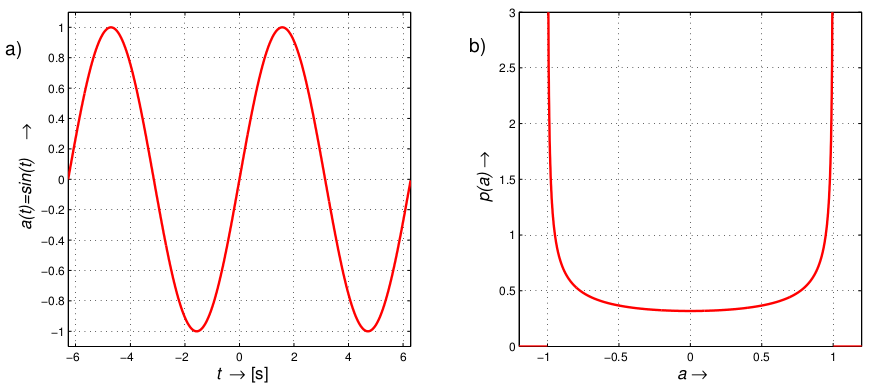
\includegraphics[width=7cm]{./bilder/amplitudenverteilung_bsp1.png}
			}
		&	\begin{minipage}[]{11cm}
				\fbox{$f(t) = sin(t)$} \\
				$t = arcsin(a)$ \\
				$\frac{dt}{da} = 2 \cdot \frac{d(arcsin(a))}{da} = 2 \cdot \frac{1}{\sqrt{1-a^2}}$ \\
				\textit{Der Faktor $2$ kommt daher, dass die Sinusfunktion nicht eindeutig ist!}\\
				\fbox{$p(a) = \frac{1}{T} \cdot \frac{dt}{da} = \frac{2}{2 \pi} \cdot \frac{1}{\sqrt{1-a^2}}$}
      		\end{minipage}
		\end{tabularx}
		}
		
	\subsection{Zentraler Grenzwertsatz}
		\begin{minipage}[]{11cm}
			$X_1, X_2, \ldots , X_n$ sind lauter identisch verteilte (nicht notwendig normalverteilt!)
			unabhängige Zufallsvariablen mit demselben Erwartungswert $\mu$ und derselben Varianz $\sigma^2$
			und mit $Z = \frac{X-\mu}{\sigma}$
		  	Dann hat die Summe
			\begin{equation}
				S_n = \frac{1}{\sqrt{n}}\sum_{i=1}^n Z_i \nonumber
			\end{equation}
			den Erwartungswert $n \mu$ und die Varianz $n \sigma^2$. \\
		  	Die damit verbundene standardisierte ($E(S_n) = 0, var(S_n) = 1$) Variable $S_n$ ist somit wie
		  	folgt definiert: \\ 
			\begin{equation}
				S_n = \frac{1}{\sqrt{n}}\sum_{i=1}^n \frac{X_i - \mu}{\sigma}
				= \frac{1}{\sqrt{n}\cdot \sigma}\left[\left(\sum\limits_{i=1}^n X_i\right) -n \mu\right]
				=\dfrac{\bar{X} - \mu}{\sigma / \sqrt{n}} \nonumber
			\end{equation}
		  	Für $\boldsymbol{n \to \infty}$ strebt die Verteilung von $S_n$ gegen die Standardnormalverteilung. \\
		  \end{minipage}
		  \begin{minipage}[]{8cm}
		  	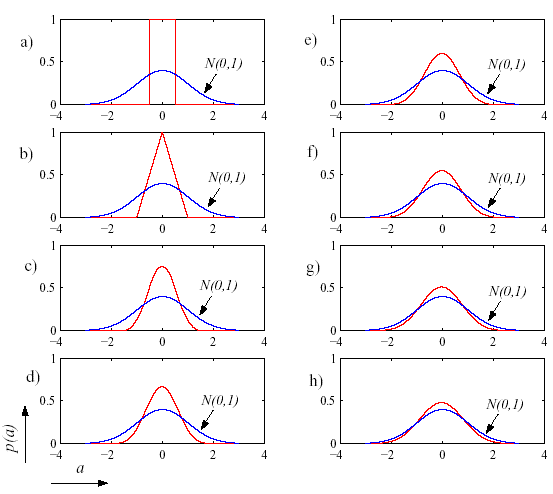
\includegraphics[width=8cm]{./bilder/grenzwertsatz.png}
		  \end{minipage}
	  	
		\subsection{Faltung \skript{34}}
		
		\begin{tabularx}{\textwidth}{lX}
			\parbox{5cm}{
				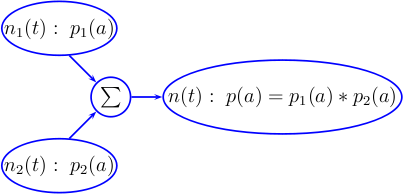
\includegraphics[width=5cm]{./bilder/faltung.png}
			}
			& 	\parbox{13cm}{
				Convolution, ``Addition zweier unabhängiger ergodischer Prozesse $n_i$'' \matlab{conv}\\
				\formel{$p(a) 	= p_1(a) \ast p_2(a)
					= p_2(a) \ast p_1(a)
					= \int\limits_{-\infty}^{\infty}p_1(\xi)\cdot p_2(a-\xi) d\xi$
				} \\
				
				\begin{itemize}
					\item Gesamtbreite der Faltung = Summe der Breiten aller Funktionen
					\item Startpunkt = Summe aller Startpunkte
					\item Endpunkt = Summe aller Endpunkte
					\item $f(t) * g(t) \ \laplace \ F(s) G(s)$
					\item $F(s) * G(s) \ \Laplace \ \frac{1}{2 \pi} f(t) g(t)$
				\end{itemize}
			}
			\\
			\textbf{Faltung zweier Normalverteilungen:}
			&
			Ergibt wieder eine Normalverteilung: \newline
			\fbox{$N(\mu_1, \sigma_1) \ast N(\mu_2, \sigma_2) = 
				N \left( \underbrace{\mu_1 + \mu_2}_{\mu} \underbrace{\sqrt{\sigma_1^2 + \sigma_2^2}}_{\sigma} \right)$}
			\\ & \\
			\textbf{Zentraler Grenzwertsatz:}
			&	Unendlich viele unabhängige Prozesse miteinander gefaltet ergibt
			(unabhängig von den einzelnen Verteilungen) eine \textbf{Normalverteilung}.
		\end{tabularx}
	
	\newpage
	\subsection{Stochastische Signale und deren Verteilungen \skript{38}}
		\rotatebox{90}{
		\begin{minipage}[]{22.5cm}
			\begin{tabular}{|c|c|c|c|c|}
			\hline
				Verteilung
			& 	\textbf{gleichverteilt}
			& 	\textbf{gaussförmig}
			& 	\textbf{sinusförmig}
			&	\textbf{exponentiell}
			\\ \hline\hline
			& 	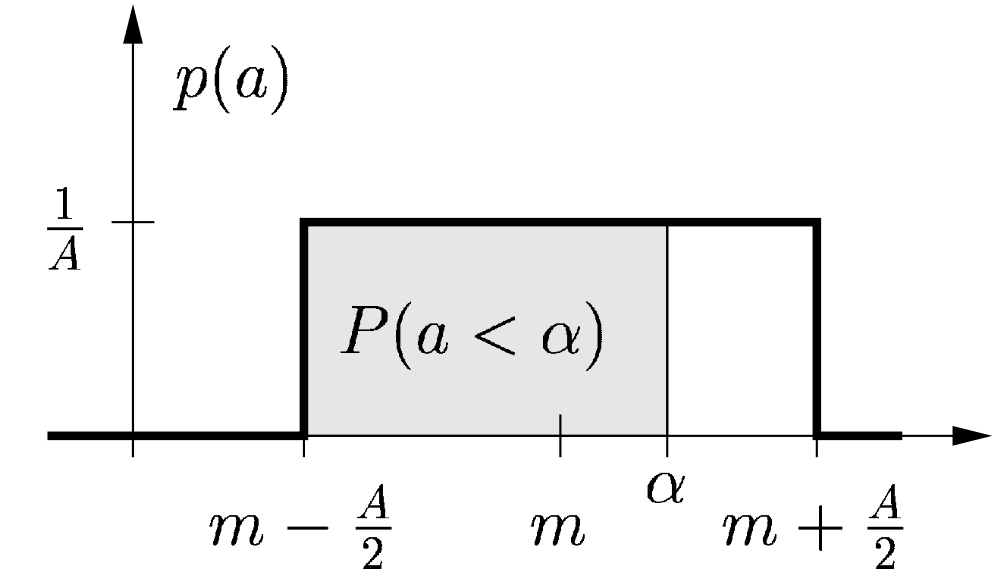
\includegraphics[width=4.3cm]{./bilder/verteilungen-gleichvert.png}
			&	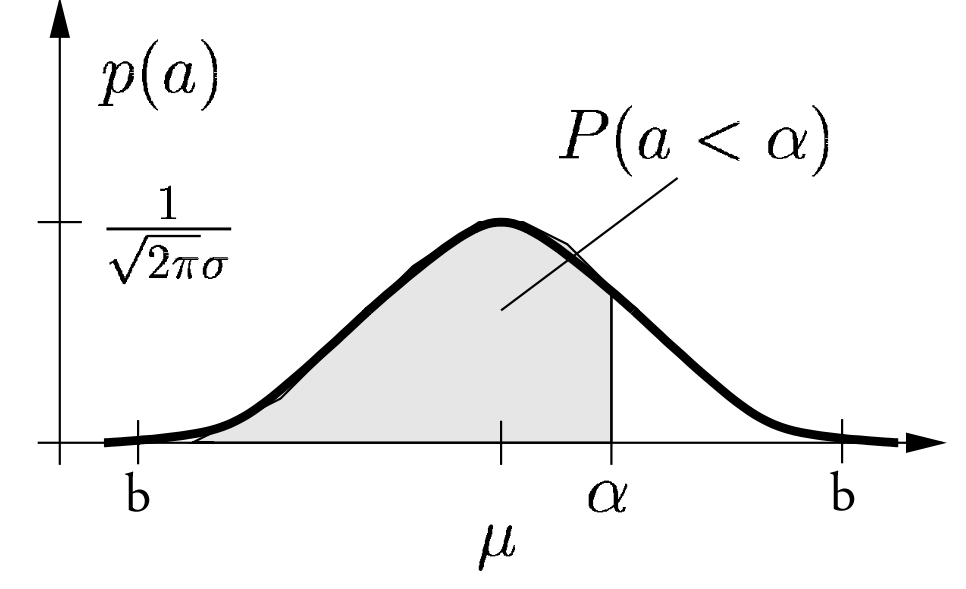
\includegraphics[width=4.3cm]{./bilder/verteilungen-gauss.png}
			&	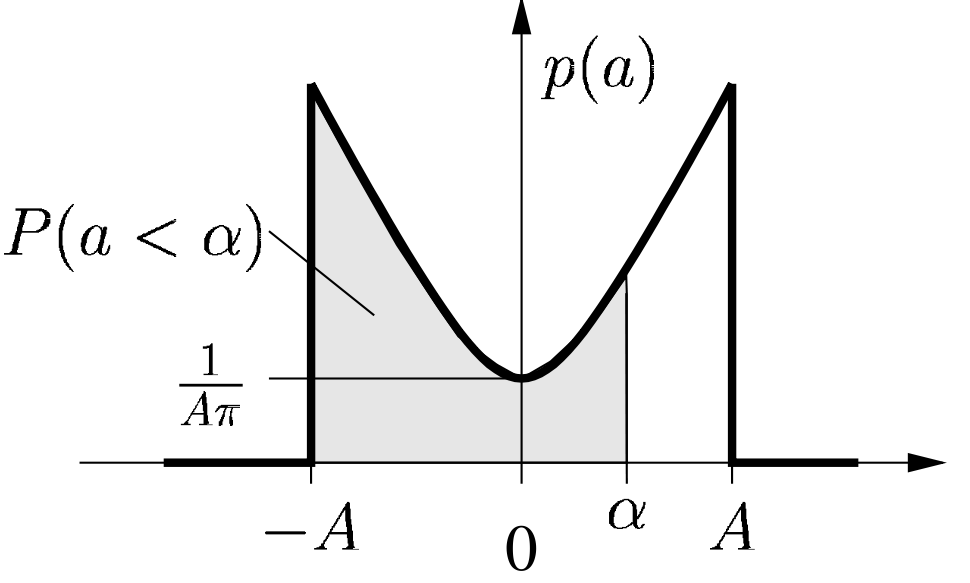
\includegraphics[width=4.3cm]{./bilder/verteilungen-sinus.png}
			&	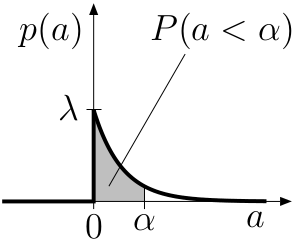
\includegraphics[width=3cm]{./bilder/verteilungen-exp.png}
			\\ \hline 
				Amplitudendichte
			& & & &
			\\ 
				$p(a)=$
			& 	$\begin{cases} \frac{1}{A}&|a-m|\leq \frac{A}{2},\\ 0&|a-m|>\frac{A}{2}.\\ \end{cases}$
			&	$\displaystyle\frac{1}{\sigma \sqrt{2\pi}}e^{\displaystyle\frac{-(a-\mu)^2}{2\sigma^2}}$
			& 	$\begin{cases} \frac{1}{\pi\sqrt{A^2-a^2}}&|a|\leq A,\\ 0&|a|>A.\\ \end{cases}$
			&	$\begin{cases} \lambda \e^{-\lambda a} & a \geq 0, \\ 0 & a<0.\\ \end{cases}$
			\\ \hline  
			 	Wahrscheinlichkeit,
			& & & &
			\\ 
				dass die Amplitude $a$
			& & & &
			\\  
				kleiner gleich $\alpha$ ist
			& & & &
			\\ 
				$P(a\!\leq\!\alpha)\!=\!\!\int\limits_{-\infty}^{\alpha}\!p(a)da=$
			&	$\begin{cases}0&\alpha<m-\frac{A}{2},\\ \frac{\alpha-(m-\frac{A}{2})}{A}&
					|\alpha-m|\leq\frac{A}{2} \\1&\alpha\geq m+\frac{A}{2}. \end{cases}$
			&	$Q\left(\frac{\displaystyle\mu-\alpha}{\displaystyle\sigma}\right)$
			&	$\begin{cases}0&\alpha\!\leq\!-A,\\ \frac{1}{\pi}\left(\frac{\pi}{2}\!+\!\sin^{-1}\!
					\left(\frac{a}{A}\right)\right)&|\alpha|\!<\!A,\\1&\alpha\geq A. \end{cases}$ 
			&	$\begin{cases} 0 & a < 0, \\ 1-\e^{-\lambda a} & a \geq 0.\\ \end{cases}$
			\\ \hline      
			& & & &
			\\ 
				linearer Mittelwert $X_0 =$
			& 	$m$
			& 	$\mu$
			& 	$0$
			&	$\dfrac{1}{\lambda}$
			\\ 
			& & & &
			\\ \hline
			& & & &
			\\
				Varianz $\operatorname{Var}(x) = $
			& 	$\dfrac{A^2}{12}$
			& 	$\sigma^2$ 
			& 	$\dfrac{A^2}{2}$ 
			&	$\dfrac{1}{\lambda^2}$
			\\
				$X^2 - X_0^2$ & & & &
			\\ \hline
			& & & &
			\\
				Leistung $X^2 =$
			& 	$m^2+\dfrac{A^2}{12}$ 
			&	$\mu^2+\sigma^2$ 
			& 	$\dfrac{A^2}{2}$
			&	$\dfrac{2}{\lambda^2}$
			\\
				$\operatorname{Var}(x) + X_0^2$
			& & & &
			\\
				(quadratischer Mittelwert) 
			& & & &
			\\ \hline
			\end{tabular}\\ \\
			\textbf{Anmerkung zur gaussförmigen Verteilung:}\\
			Im Intervall $\mu \pm 3\sigma$ sind 99,73\% aller Messwerte zu finden.
			In der Zeichung ist diese Stelle mit \textbf{b} gekennzeichnet.\\ \\
			Allgemein: \formel{$\operatorname{Var}(x) = X^2 - X_0^2$}
		\end{minipage}
		}
		\newpage

		
		
%	\subsection{Q-Funktion \skript{41}}
%	
%		\begin{tabular}{ll}
%			\parbox{6cm}{
%				Tabelle \skript{52} \\
%				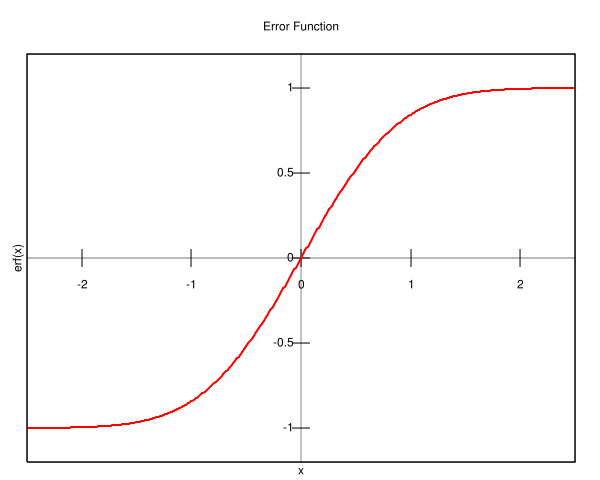
\includegraphics[width=5cm]{./bilder/q-funktion.png}
%			}
%		& 	\parbox{12cm}{
%				``Wahrscheinlichkeit eines Fehlers'' \matlab{erf, erfc} \\
%				Wenn die Resultate einer Messserie mit einer Normalverteilung mit Varianz
%				$\sigma$ und Erwartungswert $0$ auftreten, dann ist
%				$\operatorname{erf}\,\left(\,\frac{a}{\sigma \sqrt{2}}\,\right)$ die
%				Wahrscheinlichkeit, dass ein einzelner Messwert zwischen $-a$ und $a$ liegt. 
%				\\
%				\fbox{$Q(\xi) = 1-Q(-\xi) = \frac{1}{\sqrt{2\pi}}\int\limits_{\xi}^{\infty}
%				e^{-\frac{y^2}{2}}dy$} \\
%				\fbox{$Q(\xi) = \frac12 \operatorname{erfc}\left(\frac{\xi}{\sqrt2}\right)
%				= \frac12 \left(1 - \operatorname{erf}\left( \frac{\xi}{\sqrt2}\right) \right)$} \\
%			}
%		\end{tabular}
%	
%	
%	\subsubsection{Beispiel: Wahrscheinlichkeit einer Falschdetektierung eines Schwellwertdetektors \skript{40}}
%		
%		\begin{tabularx}{\textwidth}{ccX}
%			\multicolumn{2}{c}{
%				\parbox{7cm}{
%					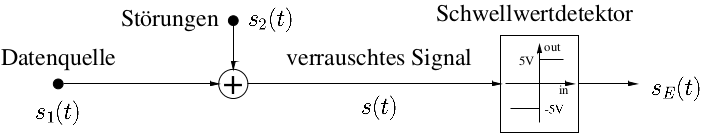
\includegraphics[width=7cm]{./bilder/schwellwertdetektor1.png}
%				}
%			}
%		&	\beispiel{\parbox{10.5cm}{
%				\textbf{Gegeben:} $\mu = 0V$, $\sigma^2 = 1V^2$\\
%				$P_{F1}$ ist die Fehlerwahrscheinlichkeit, dass 5V gesendet wurde, der Detektor sich aber für -5V entschieden hat
%				($P_{F2}$ umgekehrt).
%			}}
%		\\
%			\parbox{2.5cm}{
%				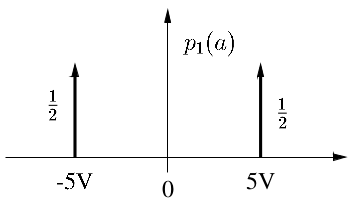
\includegraphics[width=3.5cm]{./bilder/schwellwertdetektor2.png}
%			}
%		&	\parbox{2.5cm}{
%				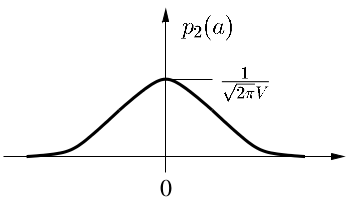
\includegraphics[width=3.5cm]{./bilder/schwellwertdetektor3.png}
%			}
%		& 	\beispiel{\parbox{10.5cm}{
%				$P_{F2} 	= \frac{1}{2} \cdot \int\limits_{0V}^{\infty V} p_2(a+5V) da
%						= \frac{1}{2} \cdot \int\limits_{0V}^{\infty V} \dfrac{1}{1V \cdot \sqrt{2 \pi}} \e^{\dfrac{-(a+5V)^2}{2 \cdot 1V^2}} da $\\
%				$P_{F1} 	= \frac{1}{2} \cdot \int\limits_{-\infty V}^{0V} p_2(a-5V) da
%						= \frac{1}{2} \cdot \int\limits_{-\infty V}^{0V} \dfrac{1}{1V \cdot \sqrt{2 \pi}} \e^{\dfrac{-(a-5V)^2}{2 \cdot 1V^2}} da $
%			}}
%		\\
%			\multicolumn{2}{c}{
%				\parbox{7cm}{
%					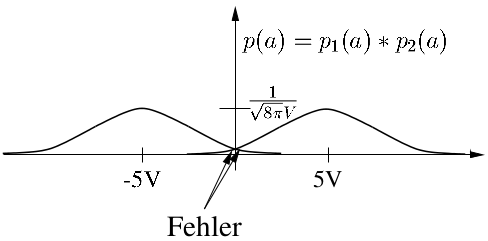
\includegraphics[width=7cm]{./bilder/schwellwertdetektor4.png}
%				}
%			}
%		&	\beispiel{\parbox{10.5cm}{
%				\textbf{Substitution:} $y = \dfrac{a-5V}{1V}$, $dy = \dfrac{da}{1V}$ \\
%				\fbox{$P_{F1} = \frac{1}{2} \cdot \int\limits_{-\infty}^{-5} \dfrac{1}{\sqrt{2 \pi}} \e^{\dfrac{-y^2}{2}} dy 
%						= \frac{1}{2} \cdot \int\limits_{5}^{\infty} \dfrac{1}{\sqrt{2 \pi}} \e^{\dfrac{-y^2}{2}} dy 
%						= \frac{1}{2} \cdot Q(5) $} \\
%				\fbox{$P_{F2} 	= \frac{1}{2} \cdot Q(5) $} \\
%				\textbf{Gesamte Fehlerwahrscheinlichkeit:}\\
%				\fbox{$P_F = P_{F1} + P_{F2} = Q(5) = 2.867 \cdot 10^{-7}$}
%			}}
%		\\ 
%		\end{tabularx}

	\subsection{Zusammenstellung einiger wichtiger Funktionen \skript{44}}
		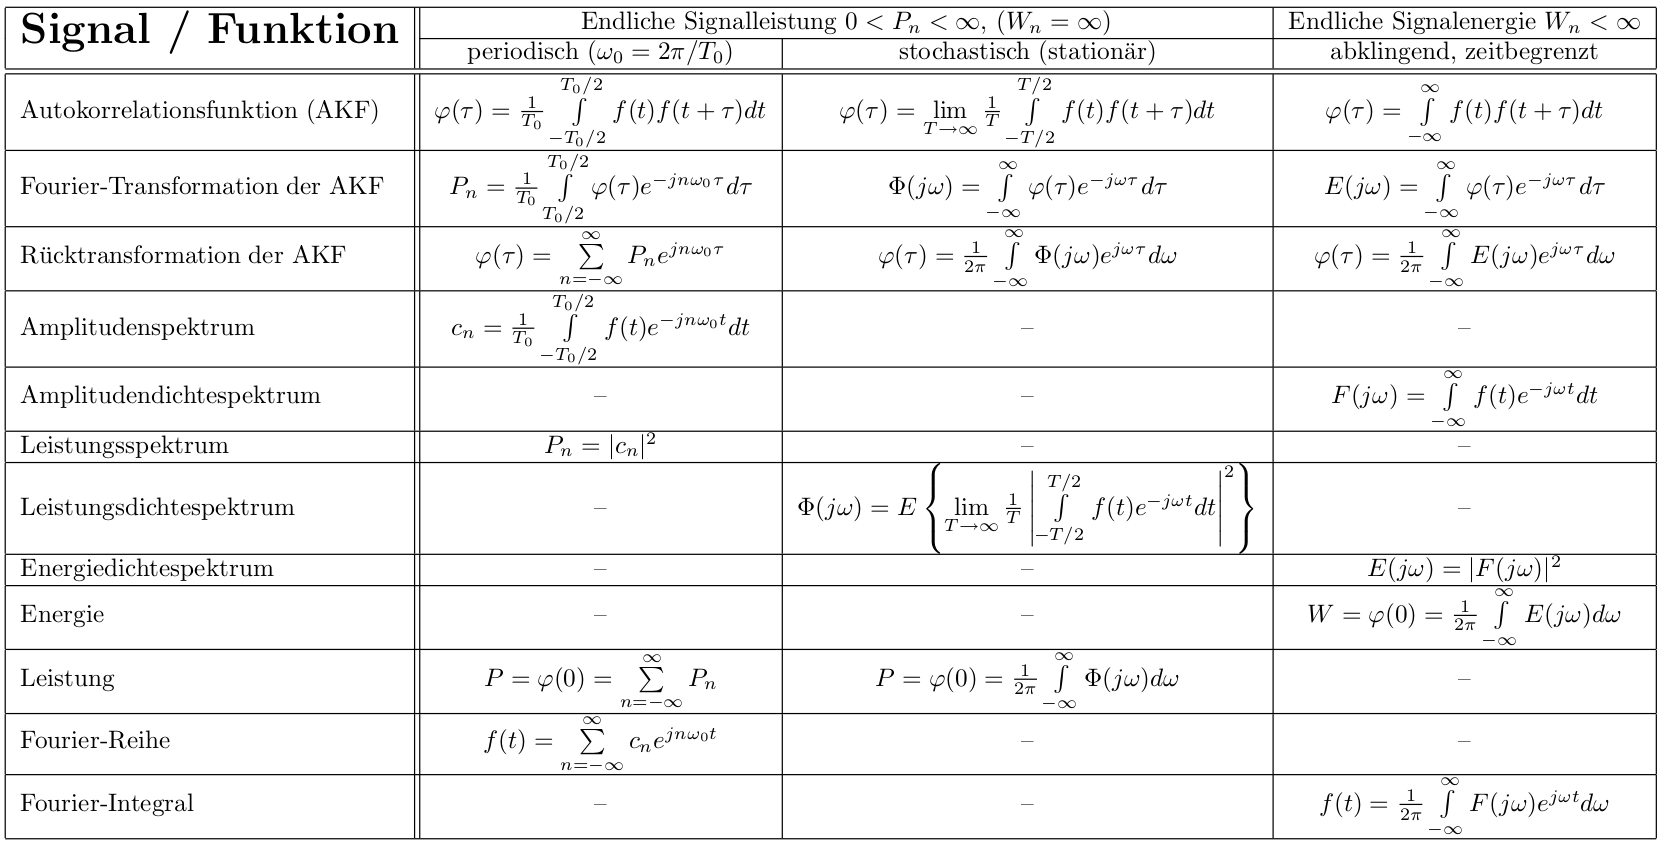
\includegraphics[width=24.5cm,angle=90]{./bilder/zusammenstellung.png}
	
\newpage
\section{Frequenzanalyse \skript{132}}

\subsection{Divere Formeln}
	\begin{tabular}{|l|l|}
		\hline
			Bessel's Theorem \skript{124} &
			$\int\limits_{-\infty}^{\infty}|f(t)|^2 dt = \frac{1}{2\pi} \int\limits_{-\infty}^{\infty}|F(j\omega)|^2d\omega$\\
		\hline
			Parseval's Theorem \skript{124} &
			$\int\limits_{-\infty}^{\infty}f(t)\cdot g^*(t)dt = \frac{1}{2\pi}\int\limits_{-\infty}^{\infty}F(j\omega)
			\cdot G^*(j\omega) d\omega$\\
		\hline
			Gibbschesph"anomen \skript{112} &
			"Uberschwinger betr"agt ca. $18\%$ der Amplitude oder ca. $9\%$ der Sprungh"ohe.\\
			& $S_{\infty} = \frac{f(x_0^+)+f(x_0^-)}{2} \qquad$ (approximiert)\\
		\hline
			Autokorrelation \skript{132} &
			$\varphi_{xx}(\tau) = \sum\limits_{k=-\infty}^{\infty}c_kc_{-k}e^{-j\frac{2\pi k}{T_0}\tau} =
			\sum\limits_{k=-\infty}^{\infty}|c_k|^2 e^{-j\frac{2\pi k}{T_0}\tau} =
			|c_0|^2 + 2\cdot \sum\limits_{k=1}^{\infty} |c_k|^2 \cdot \cos(\frac{2\pi k}{T_0}\tau)$ \\
		\hline
			Leistung \skript{119} &
			$X^2 = \sum\limits_{k=-\infty}^{\infty} |c_k|^2 = |c_0|^2 + 2\cdot \sum\limits_{k=1}^{\infty} |c_k|^2 =
			(\frac{a_0}{2})^2 + \sum\limits_{k=1}^{\infty} \frac{a_k^2 + b_k^2}{2} =
			(\frac{a_0}{2})^2 + \sum\limits_{k=1}^{\infty}\frac{A_k^2}{2}$\\
		\hline
			Bandbreitentheorem \skript{122} &
			$\Delta\omega \cdot \Delta t \geq \gamma \qquad \text{mit } \gamma \geq \frac{1}{2}$\\
		\hline
	\end{tabular}
	
\subsection{Leisungsdichtespektrum \skript{132}}
	\begin{tabular}{p{6cm} l}
		$\phi(j\omega) = \lim\limits_{T\to\infty} \frac{|F(j\omega)|^2}{T}$ &
		$\phi(j\omega)$: Leistungsdichtespektrum\\
		
		$P_n = \frac{1}{2\pi} \int\limits_{-\infty}^{\infty}\phi(j\omega)d\omega$ &
		$P_n$: normierte Leistung\\
		
		$E(j\omega) = |F(j\omega)|^2$ &
		$E(j\omega)$: Energiedichtespektrum
	\end{tabular}
	
\begin{minipage}[]{10cm}
\subsection{Wiener-Chintchine Theorem \skript{133}}
	Leistungssignal 2a: \\
	$\varphi_{xx}(t) = \frac{1}{2\pi}\int\limits_{-\infty}^{\infty}\phi(j\omega)e^{j\omega t}d\omega \; \laplace \; \phi(j\omega) = \int\limits_{-\infty}^{\infty}\varphi_{xx}(t)e^{-j\omega t} dt \nonumber $\\
	Energiesignal: \\
	$\varphi_{xx}(t) = \frac{1}{2\pi}\int\limits_{-\infty}^{\infty}E(j\omega)e^{j\omega t}d\omega \; \laplace \; E(j\omega) = \int\limits_{-\infty}^{\infty}\varphi_{xx}(t)e^{-j\omega t} dt \nonumber $\\
	Leistungssignal 2b: \\
	$\varphi_{xy}(t) = \frac{1}{2\pi}\int\limits_{-\infty}^{\infty}\phi_{xy}(j\omega)e^{j\omega t}d\omega \; \laplace \;
	\phi_{xy}(j\omega) = \int\limits_{-\infty}^{\infty}\varphi_{xy}(t)e^{-j\omega t} dt \nonumber$
\end{minipage}
\begin{minipage}[]{8cm}
\subsection{Eigenschaften von $\phi(j\omega)$}
	\begin{enumerate}
		\item	$\phi(j\omega)$ ist reell
		\item $\phi(j\omega) \geq 0$
		\item $\phi(j\omega) = \phi(-j\omega)$
		\item $P = X^2 = \varphi_{xx}(0) = \frac{1}{2\pi} \int\limits_{-\infty}^{\infty} \phi(j\omega) d\omega$
		\item $\phi(0) = \int\limits_{-\infty}^{\infty} \varphi_{xx}(\tau)d\tau$
	\end{enumerate}
\end{minipage}
\section{Systeme \skript{161}}	
	\subsection{Begriffe}
	
		\begin{tabularx}{\textwidth}{|p{4.5cm}|p{6cm}|X|}
		\hline
			\textbf{Bezeichnung}
		& 	\textbf{Beschreibung}
		& 	\textbf{Bedingung, Erkennung}
		\\ \hline
			Wirkungsfreiheit \skript{161}
		& 	Eingang des Systems hochohmig, \newline Ausgang niederohmig
		& 	Kaskadierte Systeme durch Einheitsverstärker verbunden
		\\ \hline
			Statische bzw. dynamische Systeme \skript{162}
		& 	Statisch: ohne Gedächtnis \newline 
			Dynamisch: mit Gedächtnis
		& 	Statisch: $u_2(t)$ nur vom Eingangssignal $u_1(t)$ bei $t$ abhängig \newline
			Dynamisch: $\int dt; \; \frac{d}{dt}; \; f(t \pm t_0) $
		\\ \hline
			Kausale bzw. akausale \newline Systeme \skript{164}
		& 	Kausal: Keine zukünftigen Werte \newline
			Akausal: System ''sieht in die Zukunft'' \newline
			\colorbox{yellow}{\parbox{6cm}{\textbf{Statische  und reale (physikalische) Systeme sind immer kausal!}}}
		& 	Kausal: $f(t - t_0); \int^t f(\tau) d \tau \quad (t_0 > 0)$ \newline
					$Impulsantwort:\ h(t) = 0 \ \ \forall \ t < 0 $ \newline \newline
			Akausal: $f(-t); \; f(t + t_0); \; \int^{t+t_0} f(\tau) d \tau$
		\\ \hline
			Lineare bzw. nichtlineare \newline Systeme \skript{165}
		&	Nichtlinear: Ausgangssignal kann \newline \textbf{neue Frequenzanteile}  enthalten\newline
			Linear: Ausgangssignal hat keine \newline neuen Frequenzanteile
		& 	Nichtlinear: $f^{\alpha}(t); \; \alpha + f(t); \; \alpha^{x(t)} $ \newline
			\textbf{$\Longrightarrow$ Kennlinie nicht durch Ursprung}\newline
			Linear: $S(x1+x2)=S(x1)+S(x2)$ \newline
					$S(c\cdot x)=c\cdot S(x)$
		\\ \hline
			Zeitinvariante bzw. zeitvariante Systeme \skript{170}
		& 	Zeitvariant: Von der Zeit abhängig \newline
			Zeitinvariant: Von der Zeit unabhängig
		& 	Zeitvariant: $\cos(t) x(t); t^{\alpha} x(t) \quad \text{(} \alpha \neq 0 \text{)} $ \newline
			Zeitinvariant: $S(x(t-t_0)=S(x)\cdot x(t-t_0)$
		\\ \hline 
		\end{tabularx}
		
		
		\subsubsection{Beispiele \skript{118}}

			\bgroup
			\setlength{\tabcolsep}{1.3mm}
			\begin{tabularx}{\textwidth}{|c|c|c|l|l|X|}
			\hline
				\multicolumn{3}{|c|}{\textbf{Systemtyp}}
			&	\textbf{Mathem. Form}
			&	\textbf{Beispiel (kausal)}
			&	\textbf{Beispiel (akausal)}
			\\ \hline
				statisch
			&	linear
			&	zeitinvariant
			&	$y(t) = \gamma \cdot x(t)$
			&	$y(t) = 3 \cdot x(t)$
			&	
			\\ \hline
				statisch
			&	linear
			&	zeitvariant
			&	$y(t) = \gamma(t) \cdot x(t)$
			&	$y(t) = t^2 \cdot x(t)$
			&	
			\\ \hline
				statisch
			&	nichtlinear
			&	zeitinvariant
			&	$y(t) = f \left\lbrace  x(t) \right\rbrace $
			&	$y(t) = 4 \cdot x^2(t)$
			&	
			\\ \hline
				statisch
			&	nichtlinear
			&	zeitvariant
			&	$y(t) = f \left\lbrace  x(t),t \right\rbrace $
			&	$y(t) = t \cdot x^3(t)$
			&	
			\\ \hline
				dynamisch
			&	linear
			&	zeitinvariant
			&	
			&	$y(t) = \dfrac{d^2 x(t)}{d t^2} - \dfrac{2 dx(t)}{dt}$
			&	$y(t) = \dfrac{d^2 x(t+1)}{d t^2} - \dfrac{2 dx(t)}{dt}$
			\\ \hline
				dynamisch
			&	linear
			&	zeitvariant
			&	
			&	$y(t) = cos(t) \cdot \int\limits_{-\infty}^{t} x(\tau) d\tau $
			&	$y(t) = cos(t) \cdot \int\limits_{-\infty}^{t+1} x(\tau) d\tau $
			\\ \hline
				dynamisch
			&	nichtlinear
			&	zeitinvariant
			&	
			&	$y(t) = \dfrac{d^2 x(t)}{d t^2} - \dfrac{2 dx(t)}{dt} + 1$
			&	$y(t) = \dfrac{d^2 x(t+1)}{d t^2} - \dfrac{2 dx(t)}{dt} + 1$
			\\ \hline
				dynamisch
			&	nichtlinear
			&	zeitvariant
			&	
			&	$ \ddot y(t) = cos(t) \cdot x(t-1) - 0.5$
			&	$ \ddot y(t) = cos(t) \cdot x(t+1) - 0.5$
			\\ \hline
			\end{tabularx}
			\egroup
			
			
	\subsubsection{Linearisierung von Systemen: Siehe \skript{169}}

	\subsection{Übertragungsfunktion von LTI-Systemen \skript{174}}
	
		\begin{tabular}{ll}
			\parbox{13cm}{
				$$h(t) \; \laplace \; H(s)$$
				$$s_2(t) = h(t) * s_1(t) \; \laplace \; S_2(s) = H(s) S_1(s)$$}
		& 	\parbox{5cm}{
				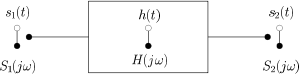
\includegraphics[width=5cm]{./bilder/utf-theorie.png}}
		\\
			\multicolumn{2}{l}{Kaskadierung von wirkungsfreien Systemen:
				$H_{total}(s) = H_1(s) H_2(s)$ bzw. bei $n$ gleichen Systemen:
				$H_{total} = (H(s))^n$}
		\\
		\end{tabular}
		
		\begin{tabular}{ll}
			\parbox{13cm}{ \beispiel{ \parbox{12cm}{
				\textbf{Beispiel}: Gesucht UTF $H(s) = \frac{Y(s)}{X(s)}$ \\
				$$H(s) = \frac{sL}{\frac{1}{sC} + sL + R} = \frac{s^2}{\frac{1}{LC} + s
					\frac{R}{L} + s^2}$$\\
				$$\Longrightarrow \text{Pole bei } s = -\frac{R}{2L} \pm j
				\sqrt{\frac{1}{LC} - \left(\frac{R}{2L}\right)^2} \quad ; \quad \text{Doppelte
				Nullstelle bei } s = 0$$
				Differentialgleichung:    $ \ddot{y}(t)+
				\frac{R}{L}\dot{y}(t)+\frac{1}{LC}y=\ddot{x}(t)$
			}}}
		& 	\parbox{5cm}{
				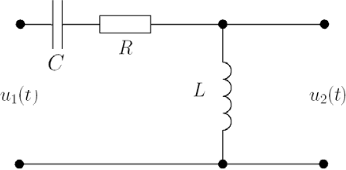
\includegraphics[width=5cm]{./bilder/utf-beispiel.png}}
		\\	
		\end{tabular}
		
		\subsubsection{Bestimmung der UTF}
		\parbox{10cm}{
			\begin{tabular}{ll}
				Bauteil & Ersatz \\
				R & R\\
				L & sL\\
				C & $\frac{1}{sC}$ \\
			\end{tabular}
			Parallelschaltung $= \frac{1}{\frac{1}{R}+\frac{1}{sL}+sC}$\\ \\}
		\parbox{8cm}{
			
			Das Potential in einem Punkt berechnet man mit $=\frac{Summe\ aller\
			Elemente\ zwischen\ Punkt\ und\ GND}{Summe\ aller\ Elemente\ der\ Kompletten\ Schaltung}$\\
			Die \textbf{Ordnung der UTF} ist die Anzahl unabhängiger Speicher (L oder C).}		
		
		\subsubsection{Beispiele von Übertragungsfunktionen (verschiedene Filter)}
		\renewcommand{\arraystretchOriginal}{1}
		\begin{tabularx}{\textwidth}{|X|c|c|c|c|}
			\hline
			{}
			&	Tiefpassfilter
			&	Hochpassfilter
			&	Bandpassfilter
			&	Allpassfilter
			\\
			{}
			&	1. Ordnung
			&	1. Ordnung
			&	2. Ordnung
			&	1. Ordnung
			\\ \hline
			{}
			&	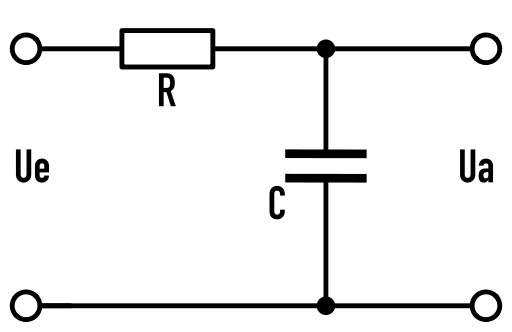
\includegraphics[width=2.5cm]{./bilder/tiefpass.png}
			&	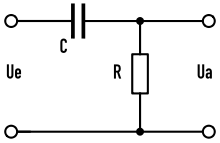
\includegraphics[width=2.5cm]{./bilder/hochpass.png}
			&	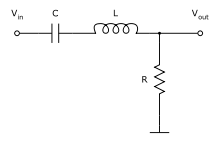
\includegraphics[width=2.5cm]{./bilder/bandpass.png}
			&	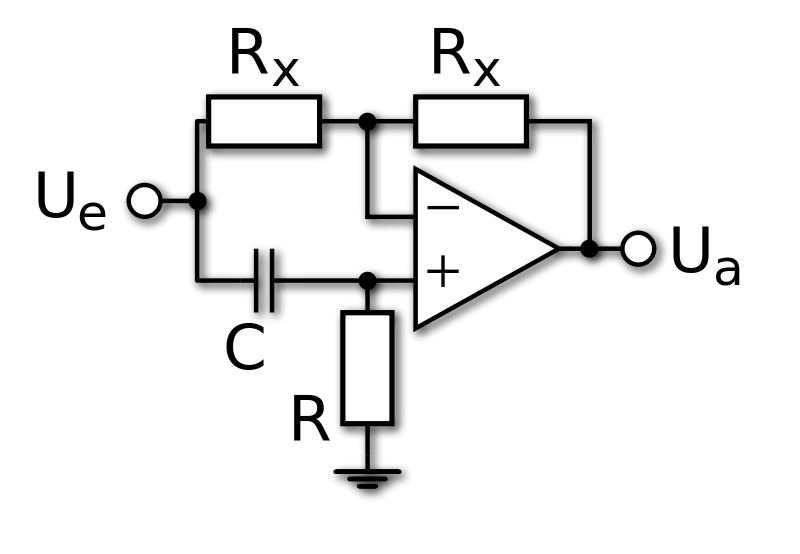
\includegraphics[width=2.5cm]{./bilder/allpass.png}
			\\ \hline & & & & \\
			Übertragungsfunktion $H(s)$
			&	$\dfrac{1}{1 + sRC}$
			&	$\dfrac{sRC}{1 + sRC}$
			&	$\dfrac{sRC}{1 + sRC + s^2 LC}$
			&	$\dfrac{sRC - 1}{sRC + 1}$
			\\ & & & & \\ \hline & & & & \\
			Amplitudengang $|H(\omega)|$
			&	$\dfrac{1}{\sqrt{1 + (\omega RC)^2}}$
			&	$\dfrac{|\omega RC|}{\sqrt{1 + (\omega RC)^2}}$
			&	$\dfrac{|\omega RC|}{\sqrt{(\omega^2 LC - 1)^2 + (\omega RC)^2}}$
			&	$1$
			\\ & & & & \\ \hline & & & & \\
			Phasengang $\varphi(\omega)$
			&	$-arctan(\omega RC)$
			&	$arctan(\dfrac{1}{\omega RC})$
			&	$-arctan(\dfrac{\omega^2 LC -1}{\omega RC})$
			&	$\pi - 2 arctan(\omega RC)$
			\\ & & & & \\ \hline & & & & \\
			Grenzfrequenz $f_c$
			&	$\dfrac{1}{2 \pi RC}$
			&	$\dfrac{1}{2 \pi RC}$
			&
			& 	
			\\ & & & & \\ \hline
			Spannung am Ausgang
			&	\multicolumn{4}{|c|}{
				$\text{Spannung am Eingang} \cdot |H(\omega)|$
			}
			\\ \hline
		\end{tabularx}
		
		\subsubsection{Berechnung des Amplituden- und Phasengangs aus der Übertragungsfunktion}
			
			$$H(j \omega) = \frac{Y(j \omega)}{X(j \omega)} = \underbrace{|H(j
			\omega)|}_{Amplitudengang} e^{j\overbrace{\Theta(\omega)}^{Phasengang}} = 
			\frac{|Y(j \omega)|}{|X(j \omega)|} e^{j (\arg(Y(j \omega)) - \arg(X(j
			\omega)))} =
			\frac{|Y(j \omega)|}{|X(j \omega)|} e^{j \left[\arctan \left(\frac{\Imag\{Y(j
			\omega)\}}{\Real\{Y(j \omega)\}} \right) - \arctan \left(\frac{\Imag\{X(j
			\omega)\}}{\Real\{X(j \omega)\}} \right)\right]}$$
			
			\begin{tabular}{ll}
				\textbf{Phasengang:} & 
				$\Theta(\omega) = \arctan \left(\frac{\Imag (H(j\omega))}{\Real (H(j\omega))}\right) \nonumber$ \\
				\textbf{Amplitudengang:} &
				$|H(j\omega)| = \frac{|Y(j\omega)|}{|F(j\omega)|} \nonumber$
			\end{tabular}
		
		
		\subsubsection{Zusammenhang zwischen Impuls- \& Einheitssprungantwort, Endwerte \skript{175}}
		
			$ \text{Einheitssprungantwort } g(t) \text{, Impulsantwort }h(t)$
			$$h(t)= \frac{d g(t)}{d t}\quad\text{bzw.}\quad
			g(t)=\int_{-\infty}^{t}h(\tau)d\tau \qquad;\qquad 
			\lim\limits_{t \rightarrow \infty}  h(t)= \lim\limits_{s \rightarrow 0} s H(s)
			\qquad;\qquad
			\lim\limits_{t \rightarrow \infty}  g(t)= \lim\limits_{s \rightarrow 0} H(s)$$
		
		
		\subsubsection{Zusammenhang zwischen Impulsantwort und Kausalität eines Systems \skript{176}}
		
			Damit ein System kausal ist, muss dessen Impulsantwort $h(t)$ für alle $t < 0$ gleich Null sein.\\
			\formel{$h(t) = 0 \ \ \forall \ t < 0 \ \ \Longrightarrow $ System kausal!}
			
	\subsection{Stabilität von LTI-Systemen \skript{177}}
		\renewcommand{\arraystretchOriginal}{1}
		\subsubsection{BIBO-Stabilität \skript{177}}
			\textit{BIBO = Bounded Input Bounded Output}\\
					Ein beliebiges System ist \textbf{BIBO-stabil}, wenn auf jedes \textbf{beschränkte Eingangssignal}
					das \textbf{Ausgangssignal} ebenfalls \textbf{beschränkt} ist.$|u_{in}(t)| < A \rightarrow |u_{out}(t)| < B$ mit $0 < A,B \in \mathbf{N} < \infty$
%	\begin{equation}
%		\int\limits_{-\infty}^{\infty} |h(t)| dt < \infty \nonumber
%	\end{equation}
		
	\subsubsection{Asymptotische Stabilität \skript{178}}
		
			\begin{tabular}{ll}
				Stabil: 
			& 	$\lim\limits_{t\rightarrow\infty} h(t) = 0$ \qquad Pole \textbf{nur} in der linken s-Halbebene.
				\textbf{Achtung: Nur \underline{Pole}, nicht \underline{Nullstellen}!!}
			\\
				Instabil: 
			& 	Mind. ein Pol in der rechten s-Halbebene oder mind. ein \textbf{mehrfacher} Pol auf der $j$-Achse der s-Ebene.
			\\
				Grenzstabil:
			& 	mindestens ein \textbf{einfacher Pol} (aber kein mehrfacher) auf der $j$-Achse, keine Pole rechts der $j$-Achse
			\end{tabular}
		
		
		\subsubsection{Stabilität mit Hurwitz-Polynom \skript{179}}
		
			Es wird jeweils das Polynom im \textbf{Nenner der Übertragungsfunktion} betrachtet:
$P(s) = a_n s^n + a_{n-1} s^{n-1} +\ldots +a_1s + a_0$ \\
Ist ein solches Polynom ein Hurwitz-Polynom, so ist das System \textbf{asymptotisch stabil}.
Handelt es sich um ein \textbf{modifiziertes Hurwitz-Polynom} so ergibt es ein
\textbf{grenzstabiles} System.\\ \\
$P(s)$ ist nur dann ein Hurwitz-Polynom, wenn folgende Bedingungen erfüllt sind:
\begin{enumerate}
	\item	alle Koeffizienten $a_i$ von $P(s)$ sind grösser als Null (und sind vorhanden).\\
				(bis zum und mit Polynomen von Grad 2, ist es notwendig, dass alle Koeffizienten positiv
				sind, damit das Polynom asymptotisch stabil ist)
	\item	alle Hurwitz-Determinanten $D_1$ bis $D_n$ sind grösser als Null\\
				\begin{align}
					D_1 &= a_{n-1} > 0 \nonumber\\
					D_2 &= \left|
						\begin{matrix}
							a_{n-1} & a_n\\
							a_{n-3} & a_{n-2}
						\end{matrix}\right| > 0 \nonumber \\
						&\vdots \nonumber \\
					D_{n-1} &= \left|
						\begin{matrix}
							a_{n-1} & a_n & 0 & 0 & \cdots & 0 \\
							a_{n-3} & a_{n-2} & a_{n-1} & a_n & 0 & 0 \\
							a_{n-5} & a_{n-4} & a_{n-3} & a_{n-2} & \cdots & 0 \\
							\vdots & \vdots & \vdots & \vdots & \ddots & 0 \\
							0 & 0 & 0 & \vdots & 0 & a_1
						\end{matrix}\right| > 0 \nonumber \\
					D_n &= a_0D_{n-1} > 0 \nonumber
				\end{align}
\end{enumerate}

\textbf{Modifiziertes Hurwitz-Polynom}\\
Nebst allen $a_i \geq 0$ müssen alle Hurwitz-Determinanten $D_1, D_2, \ldots, D_{n-2} > 0$
und $D_{n-1} = D_n = 0$ sein. \\ \\

Für Polynome $P(s) = a_n \cdot s^n + a_{n-1} \cdot s^{n-1} + \ldots + a_1 \cdot s^1 + a_0$ vom
Grad n gilt für $a_i > 0$:\\
\begin{tabular}{|l||l| l|}\hline
$N$   &   $P(s)$ ist ein Hurwitz-Polynom (stabil) &  $P(s)$ ist ein
modifiziertes Hurwitz-Polynom (grenzstabil) \\ \hline\hline
      1     &      gilt f"ur alle $P(s)$          &  $a_0=0$ \\ \hline
      2     &     gilt f"ur alle $P(s)$           &  $a_1=0$ \\ \hline
      3     &     $a_1a_2>a_0a_3$      &  $a_1a_2=a_0a_3$ \\ \hline
      4     &     $a_3(a_1a_2-a_0a_3)>a_1^2a_4$   &    $a_3(a_1a_2-a_0a_3)=a_1^2a_4$\\ \hline

      5    &     {\footnotesize $a_3a_4>a_2a_5$  und}   &     {\footnotesize $a_3a_4>a_2a_5$} \\
           &     {\footnotesize
           $(a_1a_2-a_0a_3)(a_3a_4-a_2a_5)>(a_1a_4-a_0a_5)^2$}   &  
           {\footnotesize $(a_1a_2-a_0a_3)(a_3a_4-a_2a_5)=(a_1a_4-a_0a_5)^2$} 
           
           	\\ \hline   
           			\end{tabular}\\
					
			\begin{itemize}
				\item Wenn \textbf{mindestens ein Koeffizient negativ} ist $(a_x < 0)$, dann ist das System \textbf{instabil}.
			  	\item Wenn \textbf{alle Koeffizienten negativ} sind, kann $-1$ ausgeklammert werden und in den Zähler verschoben werden\\
			  			$\Rightarrow$ \textbf{System stabil} oder \textbf{grenzstabil} %(siehe Punkt 3)
			  	\item Wenn \textbf{ein Koeffizient nicht vorhanden} ist $(a_x = 0)$, dann ist das System evtl. grenzstabil, 
			  			d.h. es ist eine \textbf{Überprüfung mit modifiziertem Hurwitz-Polynom} nötig.
			\end{itemize}

	\subsection{Phasen- \& Gruppenlaufzeit \skript{182}}
	
		\definecolor{gruppe}{rgb}{1,.75,0} % 255,192,0
		\definecolor{phase}{rgb}{1,0,0} % 255,0,0
		Die \textcolor{phase}{Phasenlaufzeit}  ist nur für reine Sinussignale bestimmbar: $\tau_P(\omega)=\frac{-\theta(\omega)}{\omega}$ \\
		Die \textcolor{gruppe}{Gruppenlaufzeit} hingegen ist für sämtliche Signale möglich: $\tau_G(\omega)=\frac{-d\theta(\omega)}{d\omega}$ \\
		\begin{center}
			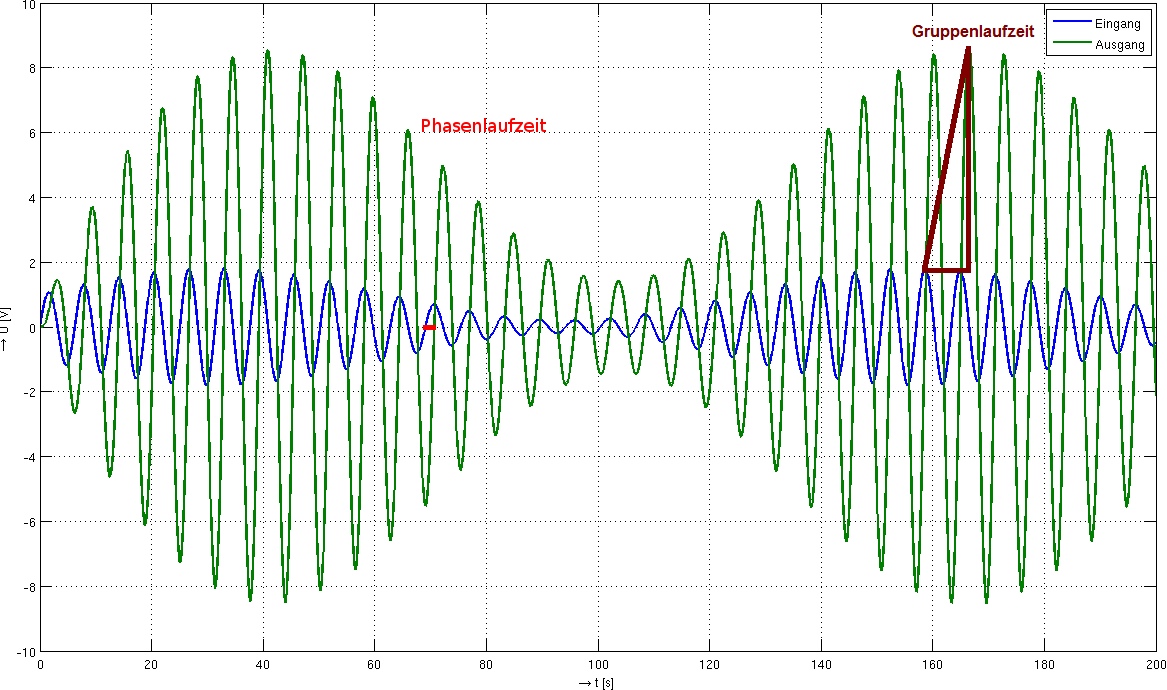
\includegraphics[width=14.5cm]{./bilder/laufzeit.png}
		\end{center}
		Eingangssignal $x(t)$ und Ausgangssignal $y(t)$ des Systems
		$H(s)=\frac{1}{s^2+0.2s+1}$. Bemerkung: $y(t)$ ist gr"osser als $x(t)$.
		
		
		\subsubsection{Signalverzögerung, Phasen- und Gruppenlaufzeit \skript{186}}
		
			Die \textbf{Signalverzögerung}, \textbf{Phasenlaufzeit} $\tau_P(\omega)$
			und \textbf{Gruppenlaufzeit} $\tau_G(\omega)$ sind identisch, wenn:
			\begin{itemize}
				\item \formel{$\theta(\omega) = -\omega \cdot t_0$}
				\item und der Amplitudengang ebenfalls konstant ist
			\end{itemize}
			
			Das heisst, $H(j \omega)$ hat die Form \formel{$H(j\omega) = a \cdot \e^{-j\omega t_0}$}. \\
			Die Signalverzögerung beträgt dann für alle Frequenzen \fbox{$t_0 = \tau_G = \tau_P$}.
		
	\subsection{Verzerrungen und Klirrfaktor \skript{187}}
	
		\subsubsection{Verzerrungen \skript{187}}
		
			\begin{tabular}{ll}
				\textbf{Lineare Verzerrungen:}
			&	\textbf{Nichtlineare Verzerrungen:}
			\\
				\parbox{9cm}{
					\begin{itemize}
						\item Erzeugen keine neuen Frequenzen
						\item z.B. Dämpfung (auch einzelner Frequenzen)
					\end{itemize}}
			&	\parbox{9cm}{
					\begin{itemize}
						\item Erzeugen neue Frequenzen
						\item z.B. Diode, Übersteuern, nichtlineare Kennlinien
					\end{itemize}}
			\\
			\end{tabular}
			
			
		\subsubsection{Klirrfaktor \skript{189}}
	
			\begin{tabularx}{\textwidth}{cX}
				\parbox{9cm}{
					Als Mass für nichtlineare Verzerrungen gilt der \textit{Klirrfaktor}. Betrachtet wird jeweils der Effektivwert am Ausgang.
					\begin{center}
						\formel{$k = \sqrt{\frac{U_2^2 + U_3^2 + \ldots + U_n^2}{U_1^2 + U_2^2 + \ldots + U_n^2}} $} $ 0 \leq k \leq 1$ 
					\end{center}
				}
			&	\parbox{9cm}{
					\begin{tabular}{ll}
						Teilklirrfaktor (frequenzselektiv):
					&	\fbox{$k_m =  \frac {U_m} {\sqrt{ U_1^2+ U_2^2 + \ldots + U_n^2} }$}
					\\
						Klirrdämpfungsmass:
					& 	\fbox{$a_k = 20 \log \left( \frac1k \right)$}
					\\
						Teilklirrdämpfungmass:
					& 	\fbox{$a_k = 20 \log \left( \frac{1}{k_m} \right)$}
					\end{tabular}
				}
			\end{tabularx}

		
		\subsubsection{Total Harmonic Distortion (THD) \skript{189}}
		
			\begin{center}
				\fbox{$\text{THD} = \sqrt{ \frac {U_2^2+ U_3^2 + \ldots + U_n^2} {U_1^2} }$}
				$\infty > \text{THD} \geq k \geq 0; \quad \text{Für kleine Verzerrungen: THD} \approx k $
			\end{center}

		
		\subsection{Verzerrungsfreie Übertragung von Signalen \skript{190}}
		
			\begin{tabularx}{\textwidth}{p{9cm}X}
				Für eine Übertragung ohne Amplitudenverzerrung \newline (konstante Amplitude über alle Frequenzen) muss gelten:
			&	$ $ \newline \fbox{$|H(j\omega)| = konstant$}
			\\
			Für eine Übertragung ohne Phasenverzerrung \newline (Phase proportional zur Frequenz) muss gelten:
			&	$ $ \newline \fbox{$\theta(\omega) = -\omega t_0$}
			\end{tabularx}\\
			\\ \\
			Für eine \textbf{verzerrungsfreie Signalübertragung} müssen \textbf{beide Kriterien} erfüllt sein!\\
			\textbf{Dann gilt:}
			\begin{itemize}
				\item \fbox{$y(t) = a \cdot x(t-t_0) \ \; \laplace \; \ Y(j\omega) = a \cdot X(j\omega) \cdot \e^{-j\omega t_0}$}
				\item \fbox{$H(j\omega) = a \cdot \e^{-j\omega t_0} = |H(j\omega)| \cdot \e^{j \theta(\omega)} \ \Laplace \ h(t) = a \cdot \delta(t-t_0)$}
			\end{itemize}	
		
	\subsection{Übertragung von stochastischen Signalen \skript{193}}
		\begin{itemize}
			\item Linearer Mittelwert und Autokorrelationsfunktion des Ausgangssignales \skript{193}
			\item Leistungsdichtespektrum \skript{193}
			\item Kreuzkorrelationen \skript{194}
			\item \textbf{Beispiel:} Leistungsdichtespektrum am Ausgang eines RC-Tiefpasses \skript{195}
		\end{itemize}
		
		
		
		
		
		
		
\newpage
%\section{Zusammenstellung Signalformen}
\begin{table}[htdp]
\begin{center}
\begin{tabular}{|c|c|c|c|c|p{6cm}|}
\hline
\textbf{Signal} & \textbf{Funktion} & \textbf{$X_0$} & \textbf{$X^2$} & \textbf{var(X)} & \textbf{Hinweise} \\

\hline
\parbox[c][2.1cm]{3.5cm}{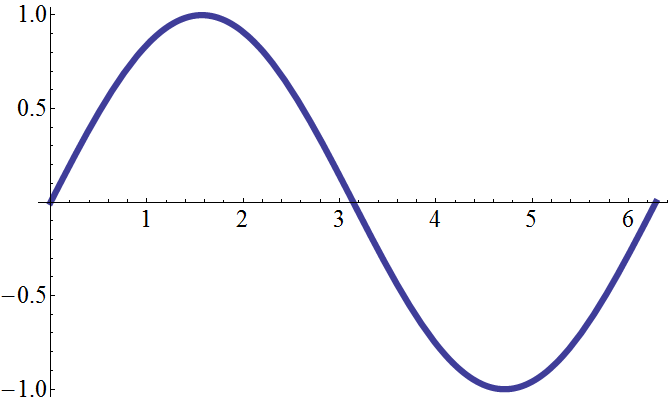
\includegraphics[height=2cm]{./bilder/Signale/Sinus.png}} &
$A\cdot\sin(t)$  & $0$ &
$\frac{A^2}{2}$ & $\frac{A^2}{2}$
&  \\

\hline
\parbox[c][2.1cm]{3.5cm}{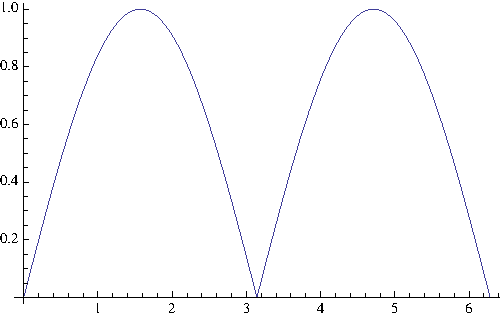
\includegraphics[height=2cm]{./bilder/Signale/absSinus.png}} &
$A\cdot|\sin(t)|$  &
$\frac{2A}{\pi}$ & $\frac{A^2}{2}$ & $\frac{A^2}{2}-\frac{4A^2}{\pi^2}$
& \\

\hline
\parbox[c][2.1cm]{3.5cm}{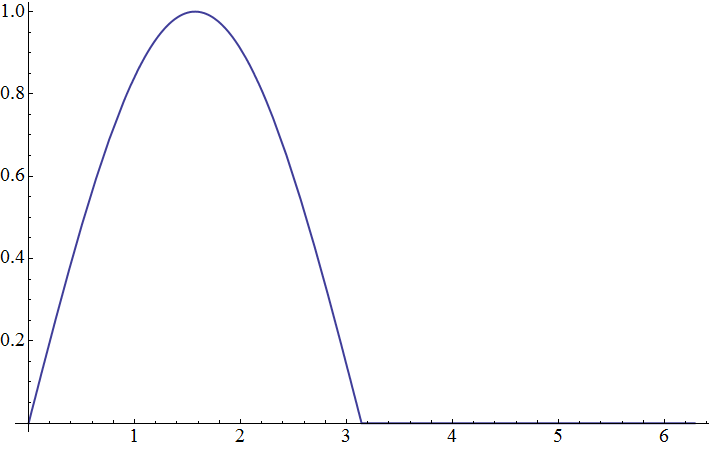
\includegraphics[height=2cm]{./bilder/Signale/Sinus_ersteWelle.png}} &
$\begin{cases} A\cdot\sin (t) & 0<t<\pi  \\ 0 & \text{True}\end{cases}$ & $\frac{A}{\pi}$ &
$\frac{A^2}{4}$ & $\frac{A^2}{4}-\frac{A^2}{\pi^2}$
& \\

\hline
\parbox[c][2.1cm]{3.5cm}{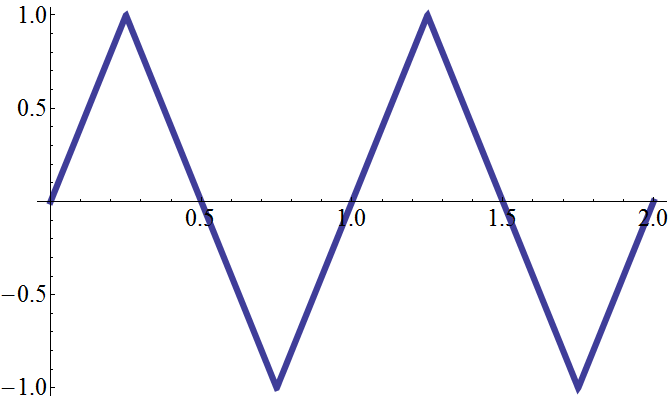
\includegraphics[height=2cm]{./bilder/Signale/Dreieck2.png}} &
$A\cdot\Lambda(t)$
& $0$ & $\frac{A^2}{3}$ &
$\frac{A^2}{3}$
& Form des $\Lambda$ egal! \\

\hline
\parbox[c][2.1cm]{3.5cm}{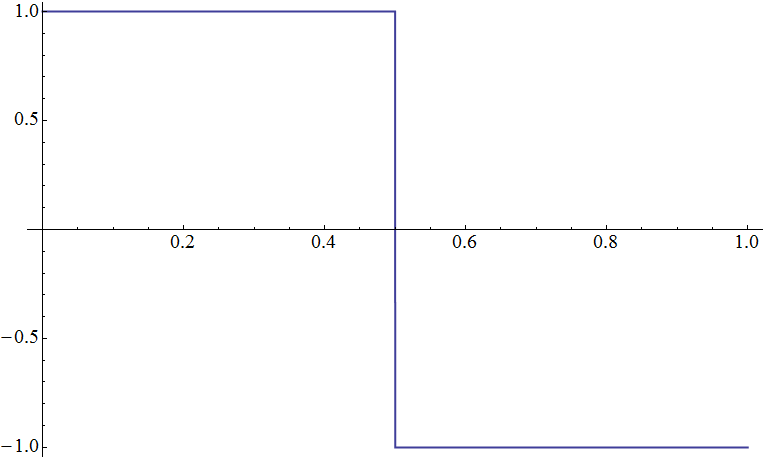
\includegraphics[height=2cm]{./bilder/Signale/UnitStep.png}} &
$A\cdot\prod(t)$
& $0$ & $A^2$ & $A^2$
& \\

\hline
\parbox[c][2.1cm]{3.5cm}{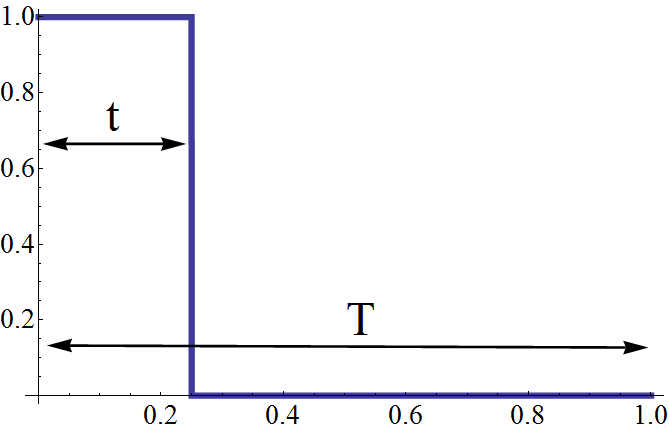
\includegraphics[height=2cm]{./bilder/Signale/StepAt_t.png}} &
$\begin{cases} A & 0<x<t \\ 0 & \text{True}\end{cases}$ 
& $A\frac{t}{T}$ &
$A^2\frac{t}{T}$ & $\frac{A^2t}{T}-\frac{A^2t^2}{T^2}$
& \\

\hline
\end{tabular}
\end{center}
\end{table}

\textbf{Allgemeine Hinweise:}
\begin{itemize}
  \item Wenn das Signal nicht symetrisch zur x-Achse ist, lässt sich der Quadratische Mittelwert einfacher über die
  Varianz berechnen. ($X^2 = X_0^2 + Var(x)$)
  \item Mittelwert \& Quadratischer Mittelwert lassen sich bei zusammengesetzten Funktionen durch zusammenzählen der
  einzelnen Stücke berechnen. Achtung: Einzelstücke richtig gewichten!
\end{itemize}
\section{Idiotenseite}
%\begin{sidewaystable}
\subsection{Ableitungen elementarer Funktionen\formelbuch{436}}
\label{unbestimmte_integrale}
\renewcommand{\arraystretchOriginal}{2.5}
\begin{tabular}{|l|l||l|l|}
  \hline
  \textbf{Funktion} & \textbf{Ableitung} & \textbf{Funktion} &
  \textbf{Ableitung}\\\hline
  $C$ (Konstante) & 0 & $\sec x$ & $\dfrac{\sin x}{\cos^2 x}$ \\
  $x$ & 1 & $\sec^{-1} x$ & $\dfrac{-\cos x}{\sin^2 x}$\\
  $x^n$ ($n\in\mathbb{R}$) & $nx^{n-1}$ & $\arcsin x \quad (|x| < 1)$ &
  $\dfrac{1}{\sqrt{1-x^2}}$\\
  $\dfrac{1}{x}$ & $-\dfrac{1}{x^2}$ & $\arccos x \quad (|x| < 1)$ &
  $-\dfrac{1}{\sqrt{1-x^2}}$\\
  $\dfrac{1}{x^n}$ & $-\dfrac{n}{x^{n+1}}$ & $\arctan x$ & $\dfrac{1}{1+x^2}$\\
  $\sqrt{x}$ & $\dfrac{1}{2\sqrt{x}}$ & arccot $x$ & $-\dfrac{1}{1+x^2}$\\
  $\sqrt[n]{x}\quad (n\in\mathbb{R}, n \neq 0, x > 0)$ &
  $\dfrac{1}{n\sqrt[n]{x^{n-1}}}$ & arcsec $x$ & $\dfrac{1}{x\sqrt{x^2-1}}$\\
  $\mathrm{e}^x$ & $\mathrm{e}^x$ & arcossec $x$ & $-\dfrac{1}{x\sqrt{x^2-1}}$\\
  $\mathrm{e}^{bx}\quad (b\in\mathbb{R})$ & $b\mathrm{e}^{bx}$ & $\sinh x$ &
  $\cosh x$\\
  $a^x\quad (a > 0)$ & $a^x\ln a$ & $\cosh x$ & $\sinh x$\\
  $a^{bx}\quad (b\in\mathbb{R}, a > 0)$ & $ba^{bx}\ln a$ & $\tanh x$ &
  $\dfrac{1}{\cosh^2 x}$\\
  $\ln x$ & $\dfrac{1}{x}$ & $\coth x \quad(x \neq 0)$ & $-\dfrac{1}{\sinh^2 x}$\\
  $\log_a{x} \quad (a > 0, a \neq 1, x > 0)$ &
  $\dfrac{1}{x}\log_a{\mathrm{e}}=\dfrac{1}{x\ln a}$ & Arsinh $x$ &
  $\dfrac{1}{\sqrt{1+x^2}}$\\
  $\lg x \quad (x > 0)$ & $\dfrac{1}{x}\lg \mathrm{e}\approx \dfrac{0.4343}{x}$
  & Arcosh $x \quad (x > 1)$ & $\dfrac{1}{\sqrt{x^2-1}}$\\
  $\sin x$ & $\cos x$ & Artanh $x \quad (|x| < 1)$ & $\dfrac{1}{1-x^2}$\\
  $\cos x$ & $-\sin x$ & Arcoth $x \quad (|x| > 1)$ & $-\dfrac{1}{x^2-1}$\\
  $\tan x \quad (x\neq(2k+1)\dfrac{\pi}{2}, k\in\mathbb{Z})$ & $\dfrac{1}{\cos^2
  x}=\sec^2 x$ & $[f(x)]^n \quad (n\in\mathbb{R})$ & $n[f(x)]^{n-1}f'(x)$\\
  $\cot x \quad (x\neq k\pi, k\in\mathbb{Z})$ & $\dfrac{-1}{\sin^2 x}=-cosec^2x$ & $\ln f(x) \quad (f(x)> 0)$ & $\dfrac{f'(x)}{f(x)}$\\
  \hline
\end{tabular}
\renewcommand{\arraystretchOriginal}{1.5}
%\end{sidewaystable}
\begin{sidewaystable}
\subsection{Einige unbestimmte Integrale\formelbuch{1074}}
\label{unbestimmte_integrale}
\begin{tabular}{|p{12cm}|p{13cm}|}
  \hline
  
    $ \int dx=x+C $ &
     $ \int{x^\alpha}dx=\frac{x^{\alpha+1}}{\alpha+1}+C,\ x \epsilon \mathbb
    R ^+,\ \alpha \epsilon \mathbb R \backslash \{ -1 \} $ \\\hline
     $ \int{\frac{1}{x}}dx=\ln \left| x \right| + C,\ x\neq0 $ &
     $ \int{e^x}dx=e^x+C $ \\\hline
     $ \int{a^x}dx=\frac{a^x}{\ln{a}}+C,\ a \epsilon \mathbb 
    R^+\backslash\{1\} $ &
     $ \int{ \sin{x}} dx = -\cos{x} + C $ \\\hline
     $ \int{\cos{x}} dx = \sin{x} + C $ &
     $ \int{\frac{dx}{\sin^2x}}=-\cot{x}+C,\ x\neq k\pi\ \mathrm{mit}\ k
    \epsilon \mathbb Z $ \\\hline
     $ \int{\frac{dx}{\cos^2x}}=\tan{x}+C,\ x\neq\frac{\pi}{2}+k\pi\
    \mathrm{mit} k \epsilon \mathbb Z $ & 
    
    %10. :
     $ \int{\sinh{x}}dx = \cosh{x}+C $ \\ \hline
     $ \int{\cosh{x}}dx = \sinh{x}+C $ &
     $ \int{\frac{dx}{\sinh^2x}}=-\coth{x}+C,\ x\neq0 $ \\\hline
     $ \int{\frac{dx}{\cosh^2x}}=\tanh{x}+C $ &
     $ \int{\frac{dx}{ax+b}} = \frac{1}{a}\ln \left|ax + b\right| + C,\
    a\neq 0,x\neq-\frac{b}{a} $ \\\hline
     $ \int{\frac{dx}{a^2x^2+b^2}}=\frac{1}{ab}\arctan{\frac{a}{b}x}+C,\
    a\neq0,\ b\neq0 $ &
     $
    \int{\frac{dx}{a^2x^2-b^2}}=\frac{1}{2ab}\ln{\left|\frac{ax-b}{ax+b}\right|}+C,\
    a\neq0,\ b\neq0,\ x\neq\frac{b}{a},\ x\neq-\frac{b}{a} $ \\\hline
     $
    \int{\sqrt{a^2x^2+b^2}}dx=\frac{x}{2}\sqrt{a^2x^2+b^2}+\frac{b^2}{2a}\ln{(ax+\sqrt{a^2x^2+b^2})}+C,\
    a\neq0,\ b\neq0 $ &
     $
    \int{\sqrt{a^2x^2-b^2}}dx=\frac{x}{2}\sqrt{a^2x^2-b^2}-\frac{b^2}{2a}\ln\left|ax+\sqrt{a^2x^2-b^2}\right|+C,\
    a\neq0,\ b\neq0,a^2x^2\geqq b^2$ \\\hline
     $
    \int\sqrt{b^2-a^2x^2}dx=\frac{x}{2}\sqrt{b^2-a^2x^2}+\frac{b^2}{2a}\arcsin\frac{a}{b}x+C,\
    a\neq0,\ b\neq0,\ a^2x^2\leqq b^2 $ &
    %20.:
     $
    \int\frac{dx}{\sqrt{a^2x^2-b^2}}=\frac{1}{a}\ln(ax+\sqrt{a^2x^2+b^2})+C,\
    a\neq0,\ b\neq0 $ \\\hline
     $
    \int\frac{dx}{\sqrt{a^2x^2-b^2}}=\frac{1}{a}\ln\left|ax+\sqrt{a^2x^2-b^2}\right|+C,\
    a\neq0,\ b\neq0,\ a^2x^2>b^2 $ &
     $ \int\frac{dx}{\sqrt{b^2-a^2x^2}}=\frac{1}{a}\arcsin\frac{a}{b}x+C,\
    a\neq0,\ b\neq0,\ a^2x^2<b^2 $ \\\hline
     Die Integrale $\int\frac{dx}{X}, \int\sqrt{X}dx,
    \int\frac{dx}{\sqrt{X}}$ mit $X=ax^2+2bx+c,\ a\neq0 $ werden durch 
    die Umformung $X=a(x+\frac{b}{a})^2+(c-\frac{b^2}{a}) $ und die
    Substitution $ t=x+\frac{b}{a} $ in die oberen 4 Zeilen
    transformiert. & $ \int\frac{xdx}{X}=\frac{1}{2a}\ln\left|X\right|-\frac{b}{a}\int\frac{dx}{X},\
    a\neq0,\ X=ax^2+2bx+c $ \\\hline
     $ \int\sin^2axdx=\frac{x}{2}-\frac{1}{4a}\cdot\sin2ax+C,\ a\neq0 $ &
     $ \int\cos^2axdx=\frac{x}{2}+\frac{1}{4a}\cdot\sin2ax+C,\ a\neq0 $ \\\hline
     $ \int\sin^naxdx=-\frac{sin^{n-1}ax\cdot\cos
    ax}{na}+\frac{n-1}{n}\int\sin^{n-2}axdx,\ n \epsilon \mathbb N,\ a\neq0 $ &
     $ \int\cos^naxdx=\frac{\cos^{n-1}ax\cdot\sin
    ax}{na}+\frac{n-1}{n}\int\cos^{n-2}axdx,\ n\epsilon \mathbb N,\ a\neq0 $
    \\\hline
     $ \int\frac{dx}{\sin ax} =
    \frac{1}{a}\ln\left|\tan\frac{ax}{2}\right|+C,\ a\neq0,\ x\neq
    k\frac{\pi}{a}\ \mathrm{mit}\ k\epsilon\mathbb Z$ &
    %30.:
     $ \int\frac{dx}{\cos
    ax}=\frac{1}{a}\ln\left|\tan(\frac{ax}{2}+\frac{\pi}{4})\right|+C,\ a\neq0,\
    x\neq\frac{\pi}{2a}+k\frac{\pi}{a}\ \mathrm{mit}\ k\epsilon\mathbb Z $
    \\\hline
     $\int\tan axdx=-\frac{1}{a}\ln\left|\cos ax\right|+C,\ a\neq0,\
    x\neq\frac{\pi}{2a}+k\frac{\pi}{a} \mathrm{mit}\ k\epsilon\mathbb Z$ &
     $\int\cot axdx=\frac{1}{a}\ln\left|\sin ax\right|+C,\ a\neq0,\ x\neq
    k\frac{\pi}{a} \mathrm{mit} k\epsilon\mathbb Z $ \\ \hline
     $ \int x^n\sin axdx=-\frac{x^n}{a}\cos ax+\frac{n}{a}\int x^{n-1}\cos
    axdx,\ n\epsilon\mathbb N,\ a\neq0 $ &
    $ \int x^n\cos axdx=\frac{x^n}{a}\sin ax-\frac{n}{a}\int x^{n-1}\sin
    axdx,\ n\epsilon\mathbb N,\ a\neq0 $ \\ \hline
     $ \int x^ne^{ax}dx=\frac{1}{a}x^ne^{ax}-\frac{n}{a}\int
    x^{n-1}e^{ax}dx,\ n\epsilon\mathbb N,\ a\neq0 $ &
     $ \int e^{ax}\sin bxdx=\frac{e^{ax}}{a^2+b^2}(a\sin bx-b\cos bx)+C,\
    a\neq0,\ b\neq0 $  \\ \hline
     $ \int e^{ax}\cos bxdx=\frac{e^{ax}}{a^2+b^2}(a\cos bx + b\sin bx)+C,\
    a\neq0,\ b\neq0 $ &
     $ \int\ln x dx = x(\ln x-1)+C,\ x\epsilon\mathbb R^+ $ \\ \hline
     $ \int x^\alpha \cdot \ln xdx =
    \frac{x^{\alpha+1}}{(\alpha+1)^2}\lbrack(\alpha+1)\ln x-1\rbrack + C,\
    x\epsilon\mathbb R^+,\ \alpha\epsilon\mathbb R\backslash\{-1\} $ & \\ \hline
    %FF1 Seite 496
    
\end{tabular}
\end{sidewaystable}
\begin{sidewaystable}
\subsection{Eigenschaften unterschiedlicher Schwingungsformen}
\begin{center}
\begin{tabular}{|l|c|c|c|c|c|c|c|c|}
\hline
	Schwingungsform & Funktion & Gleichrichtwert & Formfaktor &
	Effektivwert & Scheitelfaktor & \textbf{$X_0$} & \textbf{$X^2$} & \textbf{var(X)} \\
\hline
	Formel &
	&
	$\overline{\left|x\right|} = \frac1T\int_{0}^{T}\left| x(t)\right|dt$&
	$\frac{X}{\overline{\left|x\right|}}$&
	$X = \sqrt{X^2} = \sqrt{\frac{1}{T} \int\limits ^{t_0+T}_{t_0}{x^2(t)dt}}$&
	$k_{s}=\frac{X_{\mathrm{max}}}{X_{\mathrm{eff}}}$&
	&
	&
	\\
\hline
	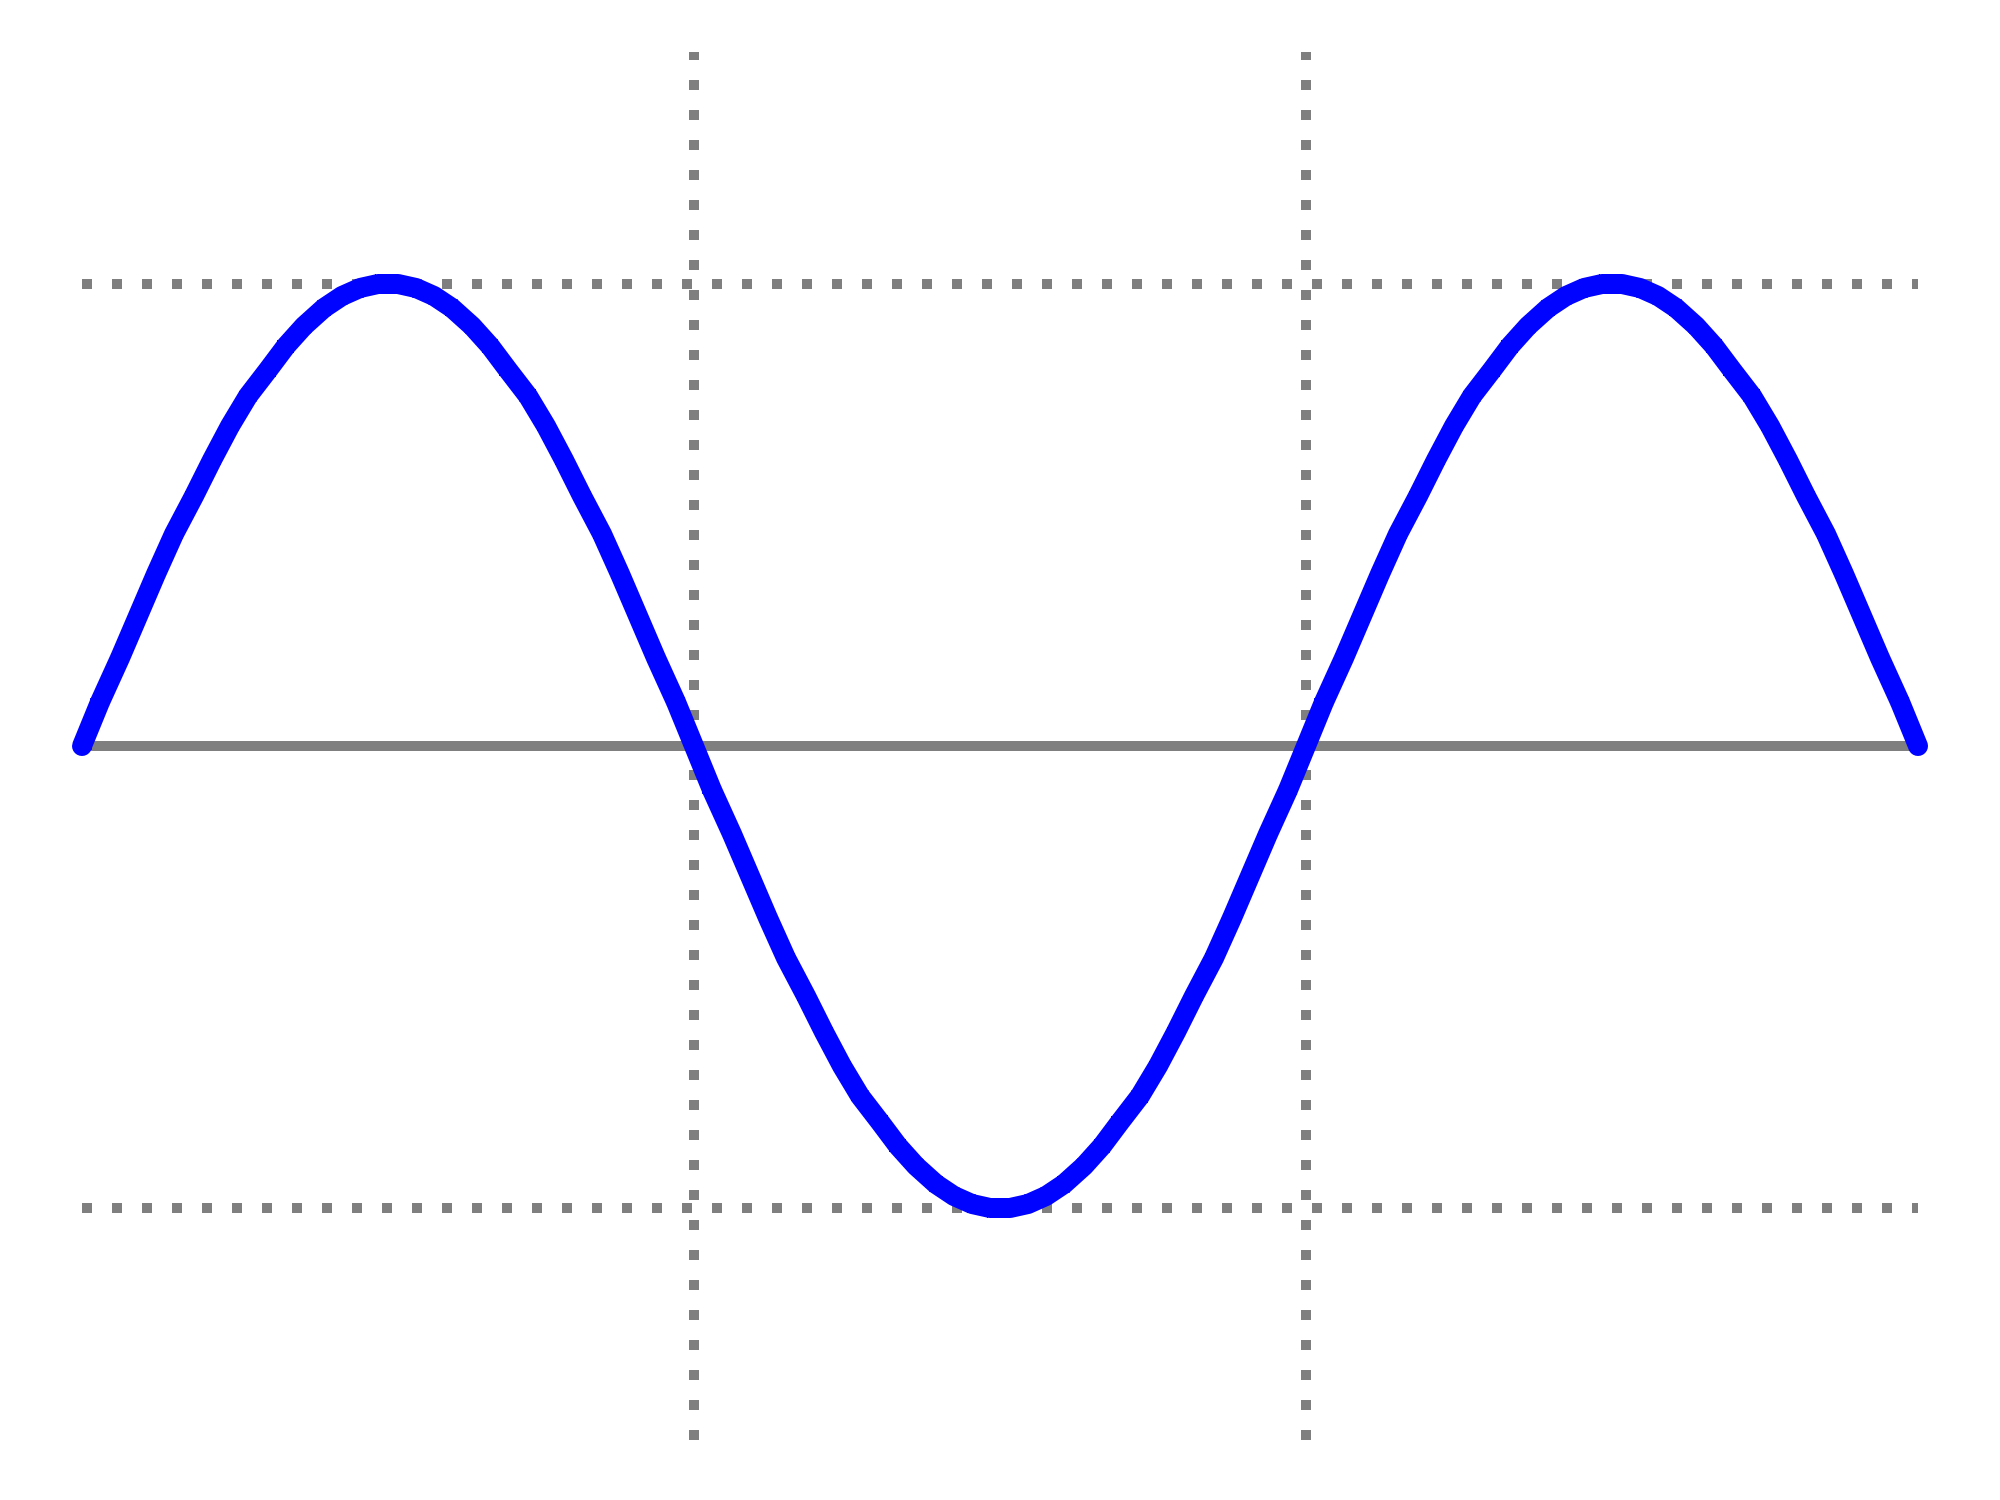
\includegraphics[width=2cm]{table/images/table_sine_wave.png} &
	$A\cdot\sin(t)$ &
	$\frac{2}{\pi} \approx 0.637$ &
	$\frac{\pi}{2\sqrt{2}} \approx 1.11$ &
	$\frac{1}{\sqrt{2}}\approx 0.707$ &
	$\sqrt{2}\approx 1.414$ &
	$0$ &
	$\frac{A^2}{2}$ &
	$\frac{A^2}{2}$ \\
\hline	
	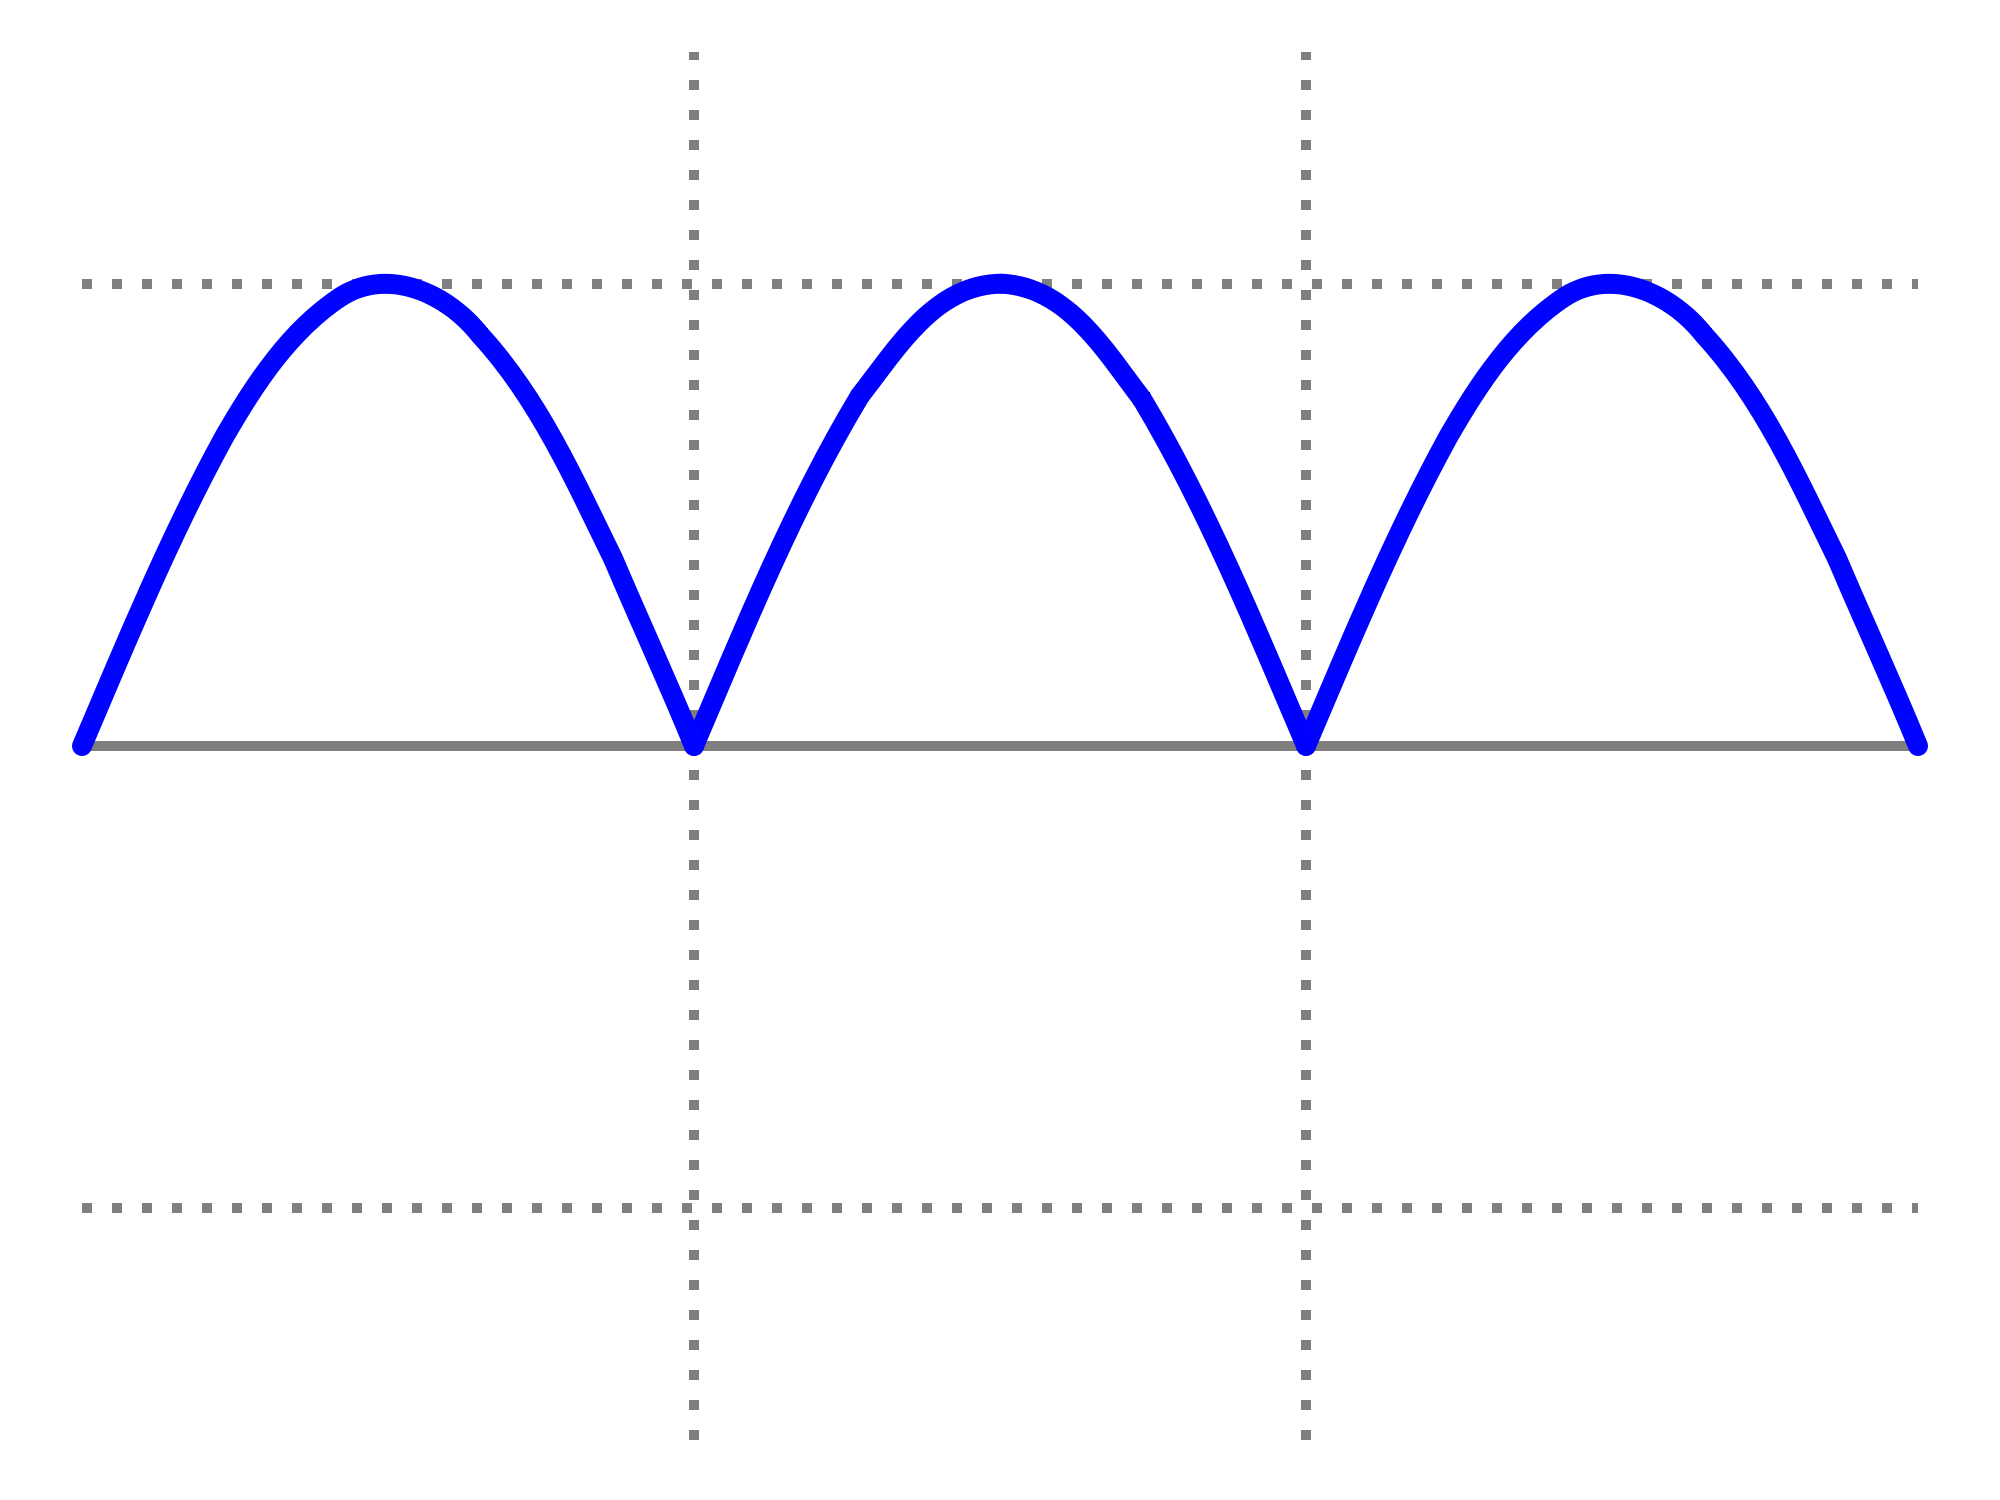
\includegraphics[width=2cm]{table/images/table_full-wave_rectified_sine.png} &
	$A\cdot|\sin(t)|$ &
	$\frac{2}{\pi} \approx 0.637$ &
	$\frac{\pi}{2\sqrt{2}} \approx 1.11$ &
	$\frac{1}{\sqrt{2}} \approx 0.707$ &
	$\sqrt{2} \approx 1.414$  &
	$\frac{2A}{\pi}$ & $\frac{A^2}{2}$ & $\frac{A^2}{2}-\frac{4A^2}{\pi^2}$
	\\
\hline
	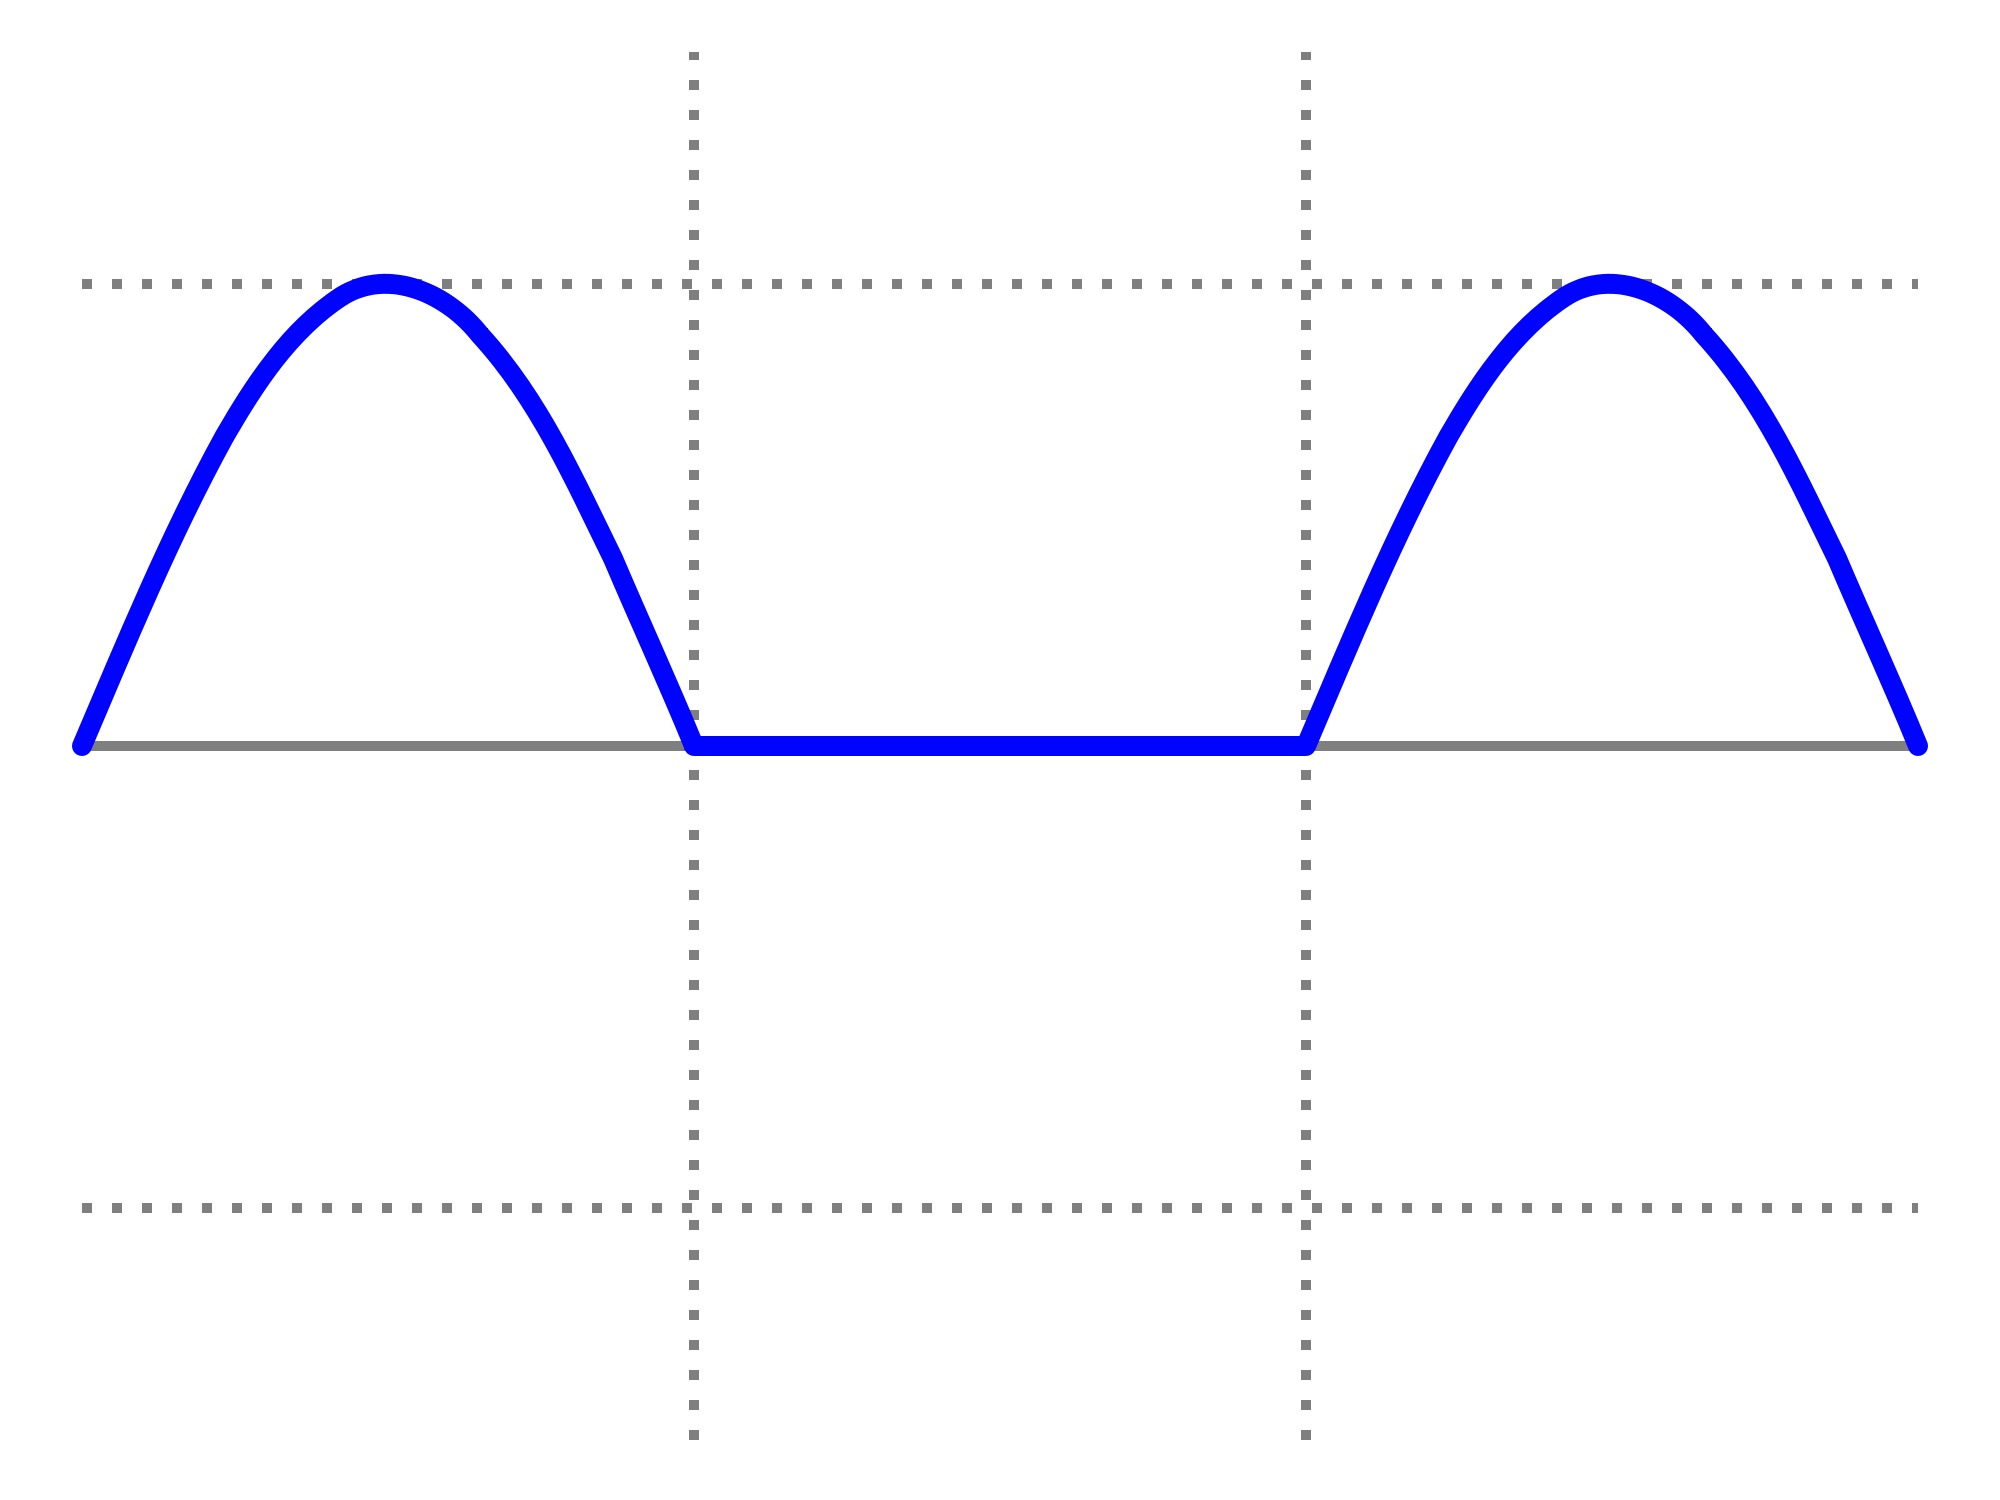
\includegraphics[width=2cm]{table/images/table_half-wave_rectified_sine.png} &
	$\begin{cases} A\cdot\sin (t) & 0<t<\pi  \\ 0 & \text{True}\end{cases}$ &
	$\frac{1}{\pi}\approx 0.318$ &
	$\frac{\pi}{2}\approx 1.571$ &
	$\frac{1}{2} = 0.5$	&
	2  &
	$\frac{A}{\pi}$ &
	$\frac{A^2}{4}$ & $\frac{A^2}{4}-\frac{A^2}{\pi^2}$
	\\
\hline
	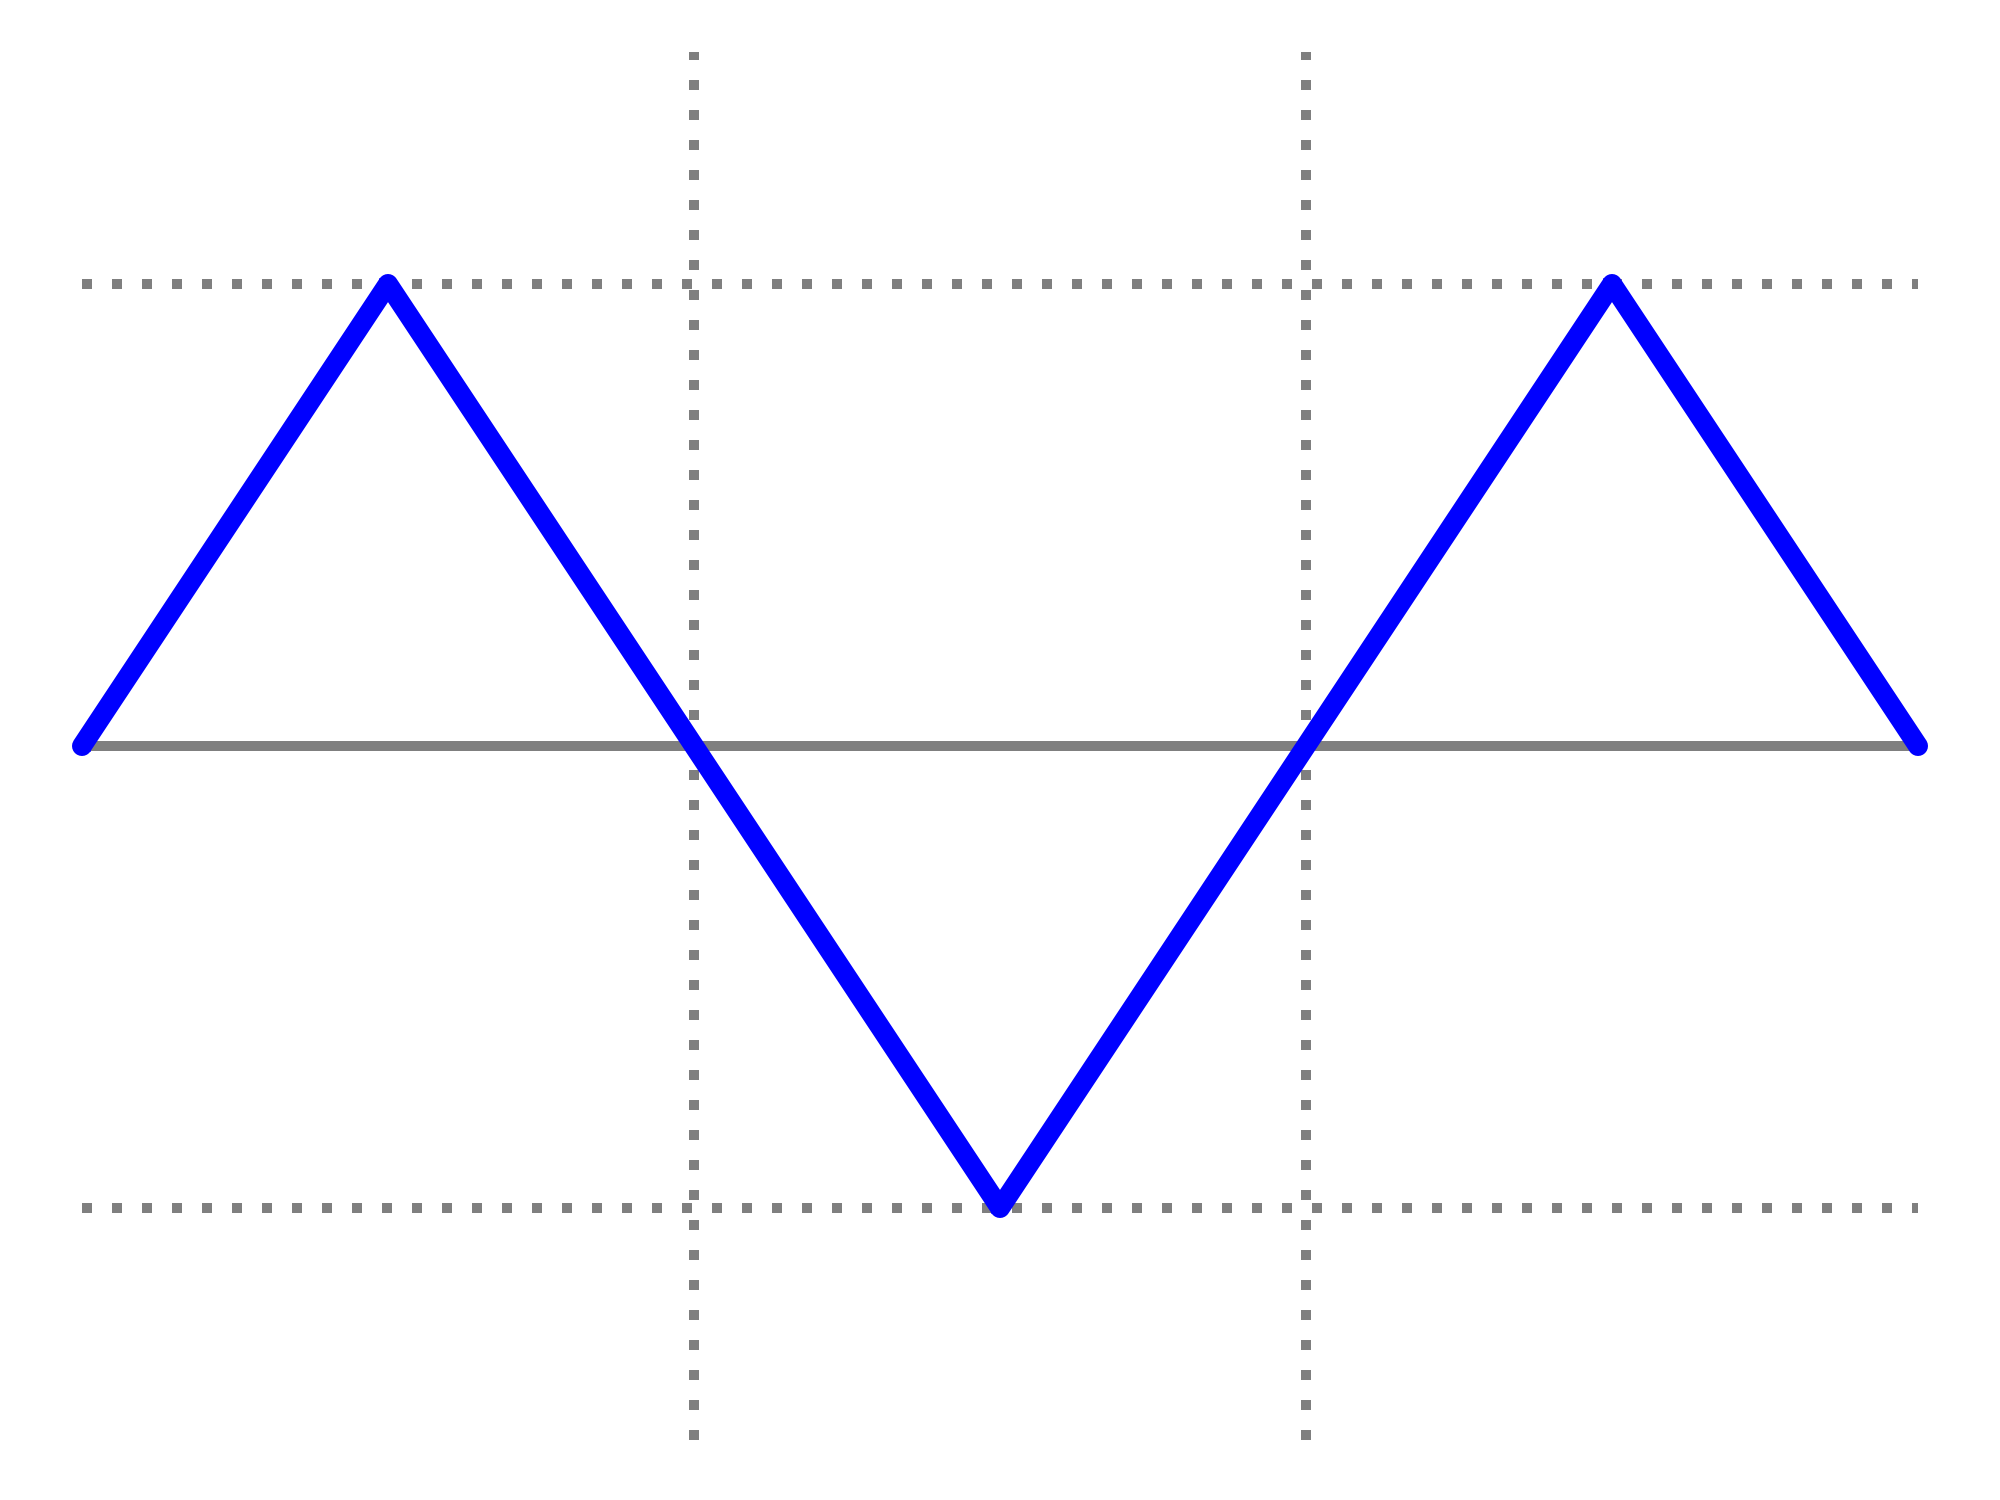
\includegraphics[width=2cm]{table/images/table_triangle_wave.png} &
	$A\cdot\Lambda(t)$ &
	$\frac{1}{2}= 0.5$ &
	$\frac{2}{\sqrt{3}}\approx 1.155$ &
	$\frac{1}{\sqrt{3}}
	\approx 0.557$ &
	$\sqrt{3} \approx 1.732$ &
	$0$ &
	$\frac{A^2}{3}$ &
	$\frac{A^2}{3}$ \\
\hline	
	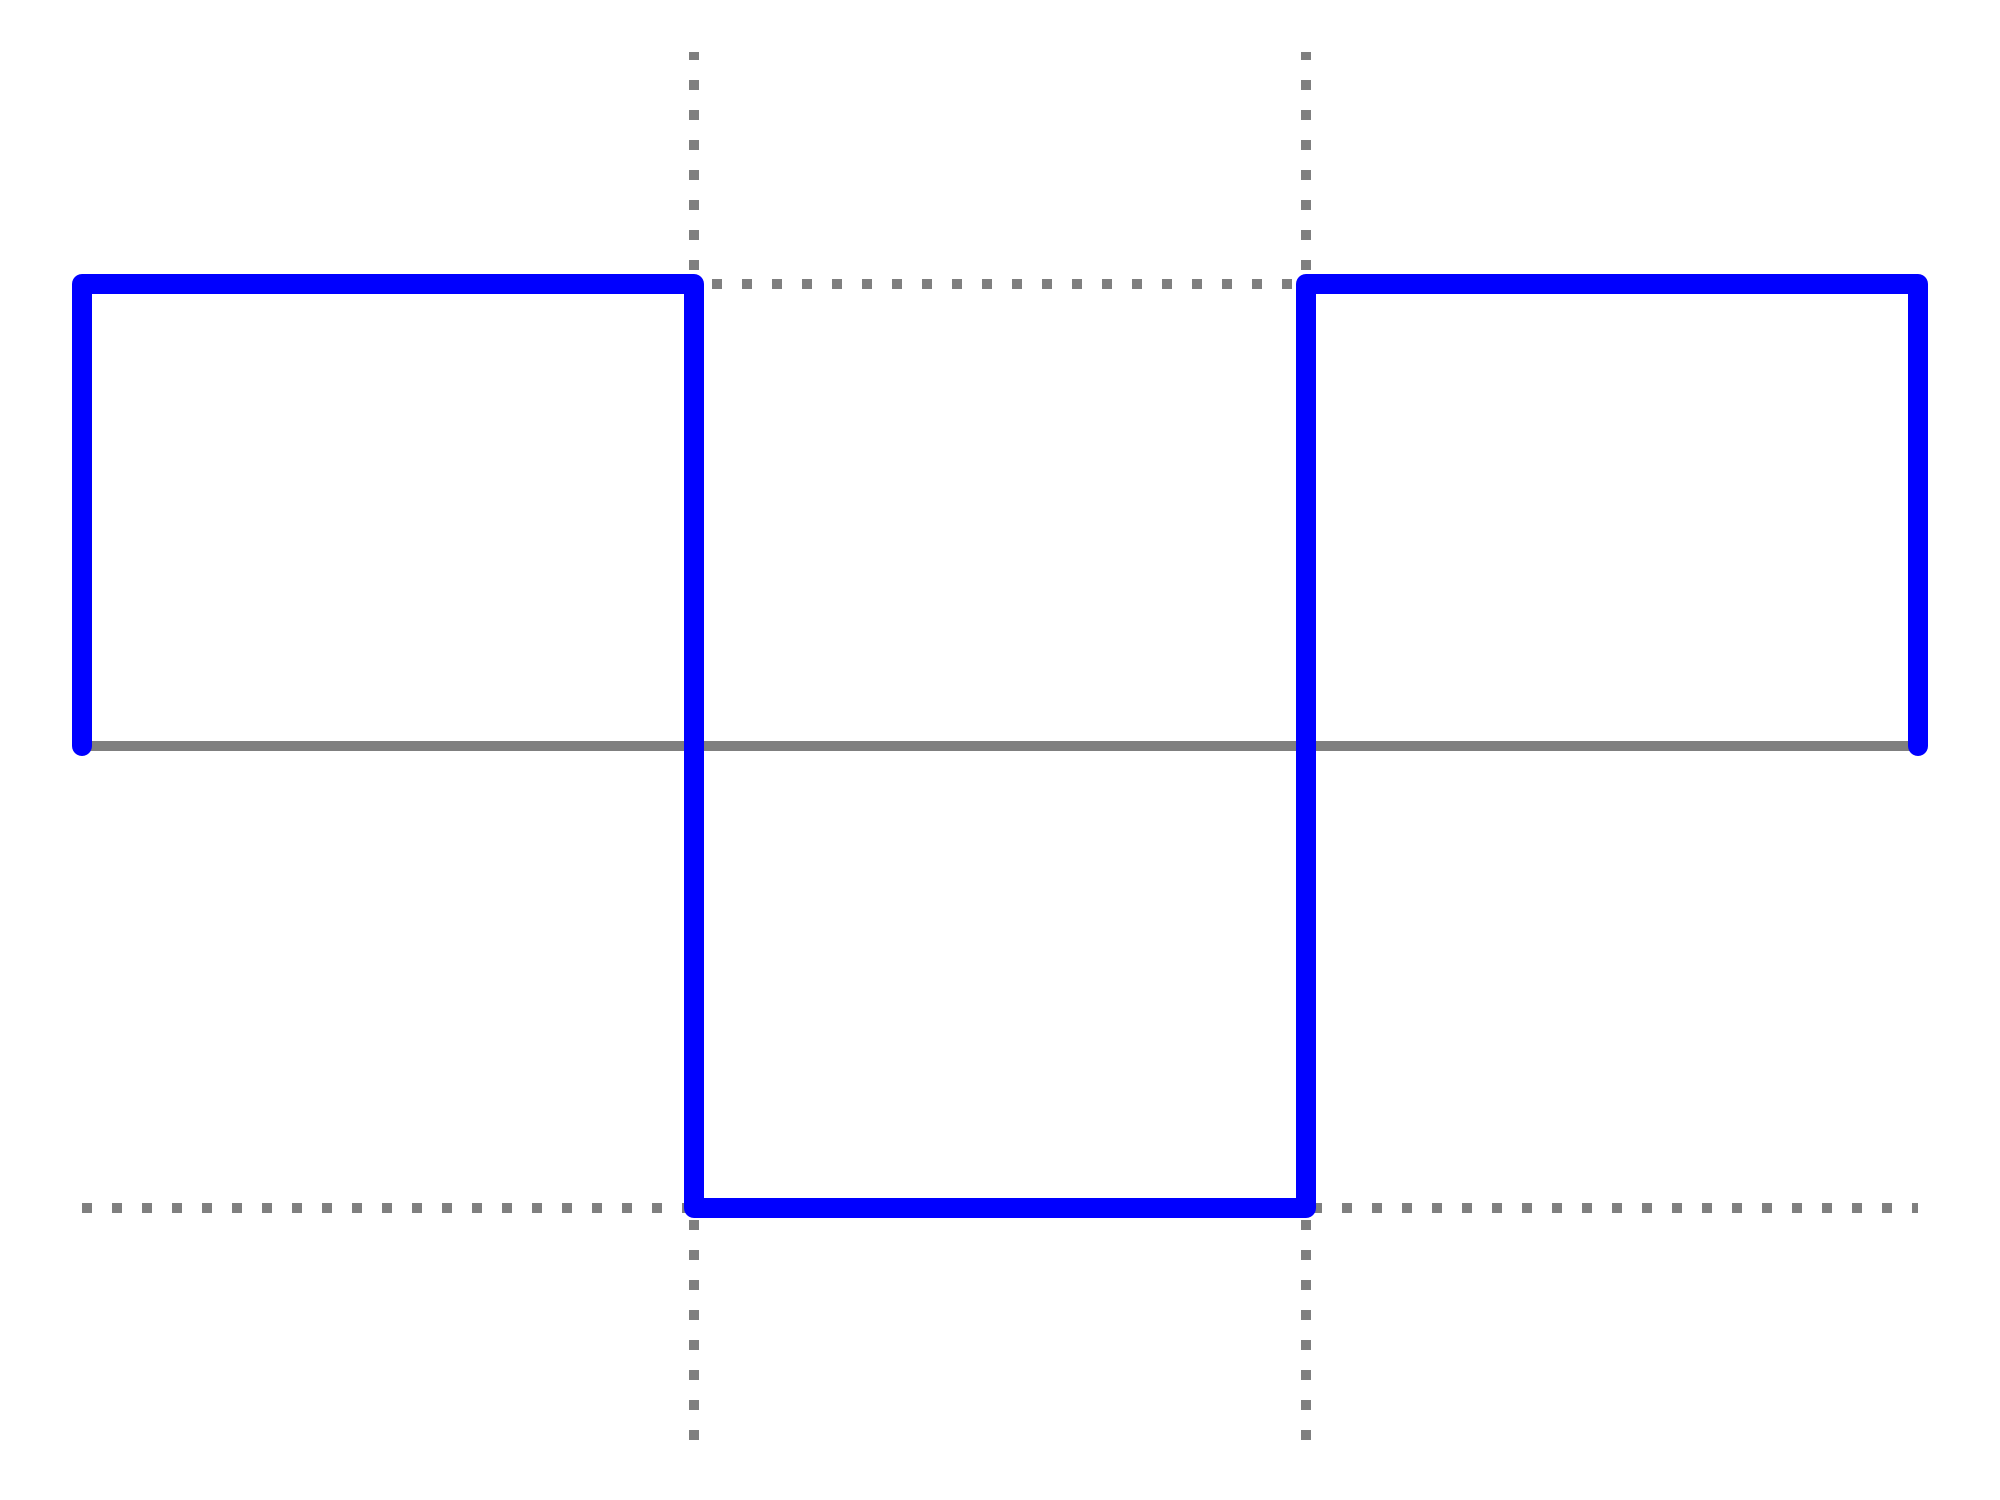
\includegraphics[width=2cm]{table/images/table_square_wave.png} &
	$\begin{cases} A & 0<x<t \\ 0 & \text{True}\end{cases}$ &
	$1$ &
	$1$ &
	$1$ &
	$1$ &
	$0$ &
	$A^2$ &
	$A^2$ \\
\hline	
	DC&
	1&
	$1$ &
	$1$ &
	$1$ &
	$1$  &
	-&
	-&
	-\\
\hline	
	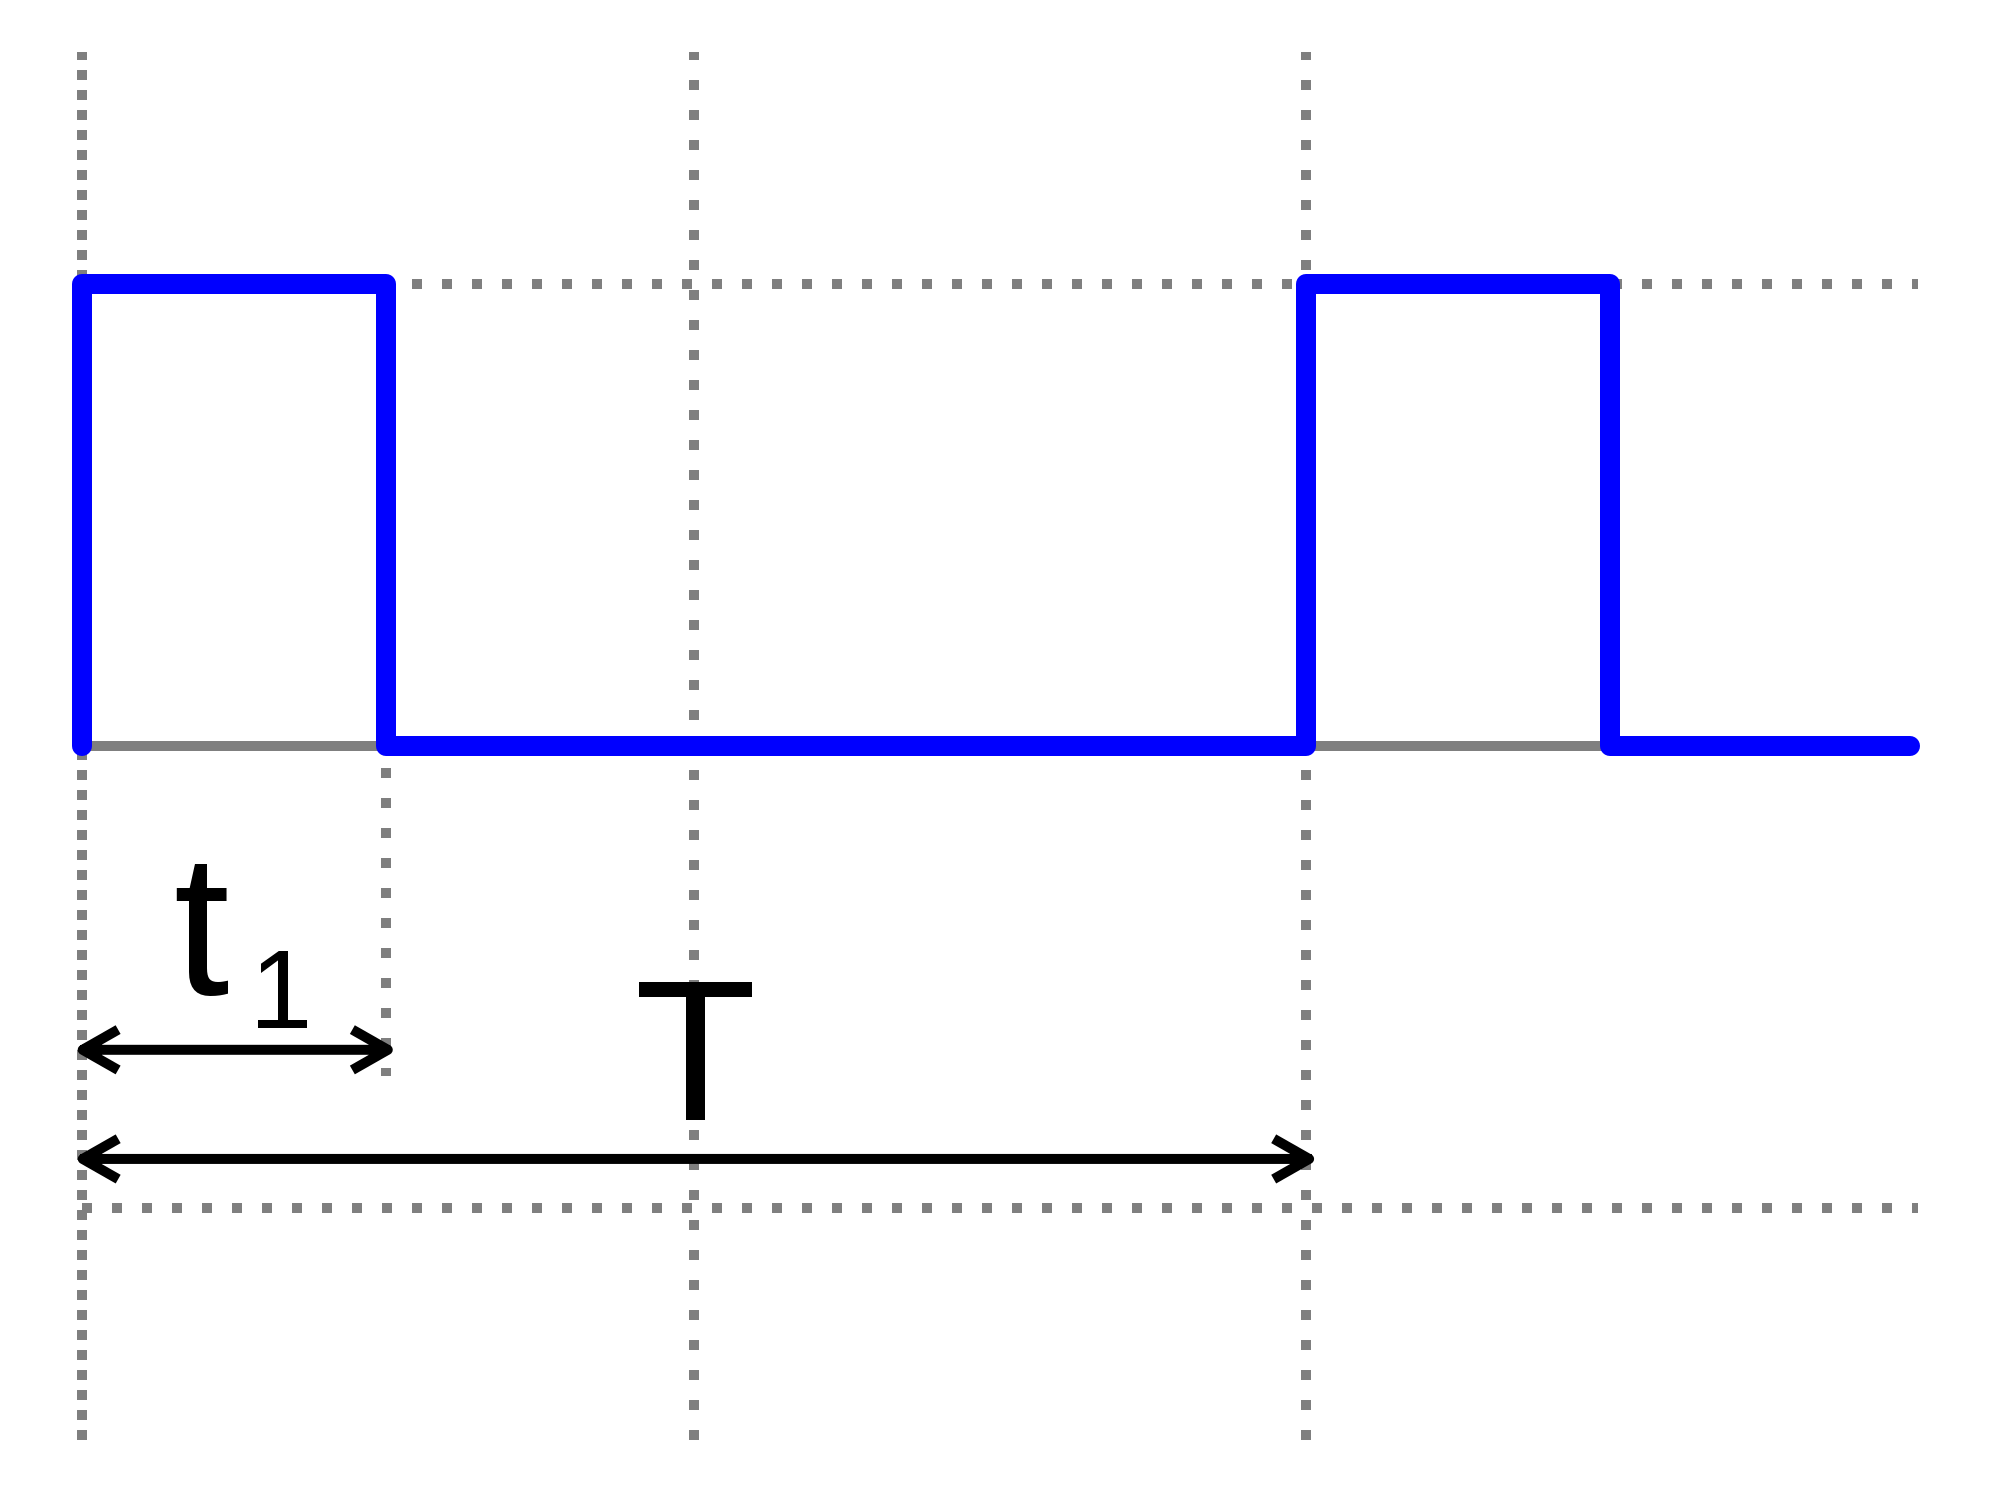
\includegraphics[width=2cm]{table/images/table_pulse_wide_wave.png} &
	&
	$\frac{t_1}{T}$ & $\sqrt{\frac{T}{t_1}}$ & $\sqrt{\frac{t_1}{T}}$ & $\sqrt{\frac{T}{t_1}}$ &
	$A\frac{t}{T}$ &
	$A^2\frac{t}{T}$ &
	$\frac{A^2t}{T}-\frac{A^2t^2}{T^2}$\\
\hline
\end{tabular}
\end{center}
\end{sidewaystable}


%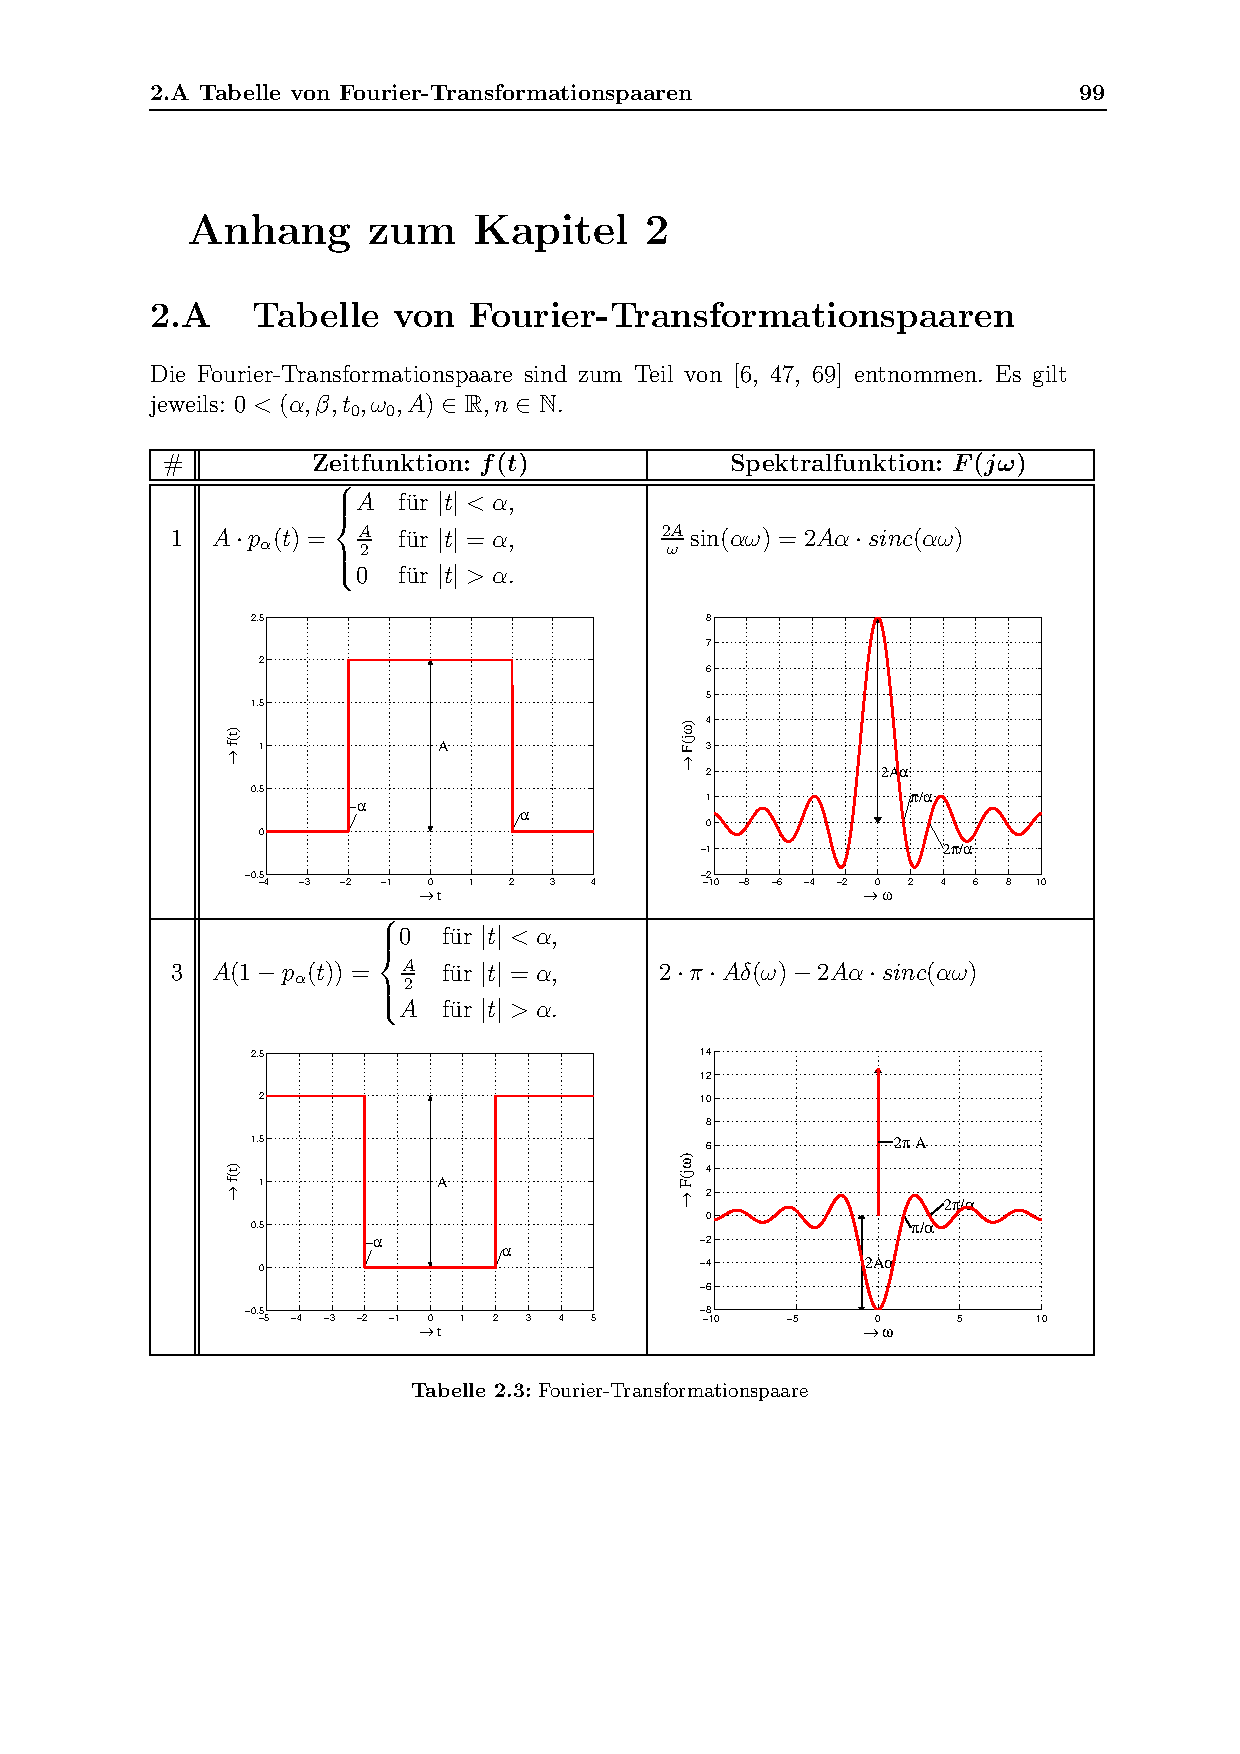
\includepdf[pages={1-9}]{Tabellen.pdf}

\end{document}
